\documentclass{article}
\usepackage[T1]{fontenc}
\usepackage{tgtermes}
\usepackage{adjustbox}
\usepackage{csquotes}
\usepackage{booktabs}
\usepackage{graphicx}
\usepackage{epstopdf}
\usepackage{subcaption}
\usepackage[hidelinks]{hyperref}
\usepackage[legalpaper, margin=1in]{geometry}
\usepackage{listings}
\usepackage{xcolor}  	%高亮使用的颜色
\usepackage{appendix}
\usepackage{multirow}
\usepackage{tabularx} % If you choose to use it for adjustable-width columns
\usepackage{lscape}   % For landscape orientation of wide tables
\usepackage{float}
\usepackage{aligned-overset}
\usepackage{bm}
\usepackage{minipage-marginpar}
\definecolor{commentcolor}{RGB}{85,139,78}
\definecolor{stringcolor}{RGB}{206,145,108}
\definecolor{keywordcolor}{RGB}{34,34,250}
\definecolor{backcolor}{RGB}{220,220,220}
\DeclareUnicodeCharacter{2064}{}
\usepackage{accsupp}	
\newcommand{\emptyaccsupp}[1]{\BeginAccSupp{ActualText={}}#1\EndAccSupp{}}
\lstset{						%高亮代码设置
	language=python, 					%Python语法高亮
	linewidth=0.9\linewidth,      		%列表list宽度
	%basicstyle=\ttfamily,				%tt无法显示空格
	commentstyle=\color{commentcolor},	%注释颜色
	keywordstyle=\color{keywordcolor},	%关键词颜色
	stringstyle=\color{stringcolor},	%字符串颜色
	%showspaces=true,					%显示空格
    breaklines,%自动换行
    columns=flexible,
	numbers=left,						%行数显示在左侧
	numberstyle=\tiny\emptyaccsupp,		%行数数字格式
	numbersep=5pt,						%数字间隔
	frame=single,						%加框
	framerule=0pt,						%不划线
	escapeinside=@@,					%逃逸标志
	emptylines=1,						%
	xleftmargin=3em,					%list左边距
	backgroundcolor=\color{backcolor},	%列表背景色
	tabsize=4,							%制表符长度为4个字符
	gobble=4							%忽略每行代码前4个字符
}

\title{CS7DS3 Main Assignment\\[1ex] 
\textit{Wines}}

\author{Kaiyu Chen\\23330889\\\href{mailto:chenka@tcd.ie}{chenka@tcd.ie}}
\date{%
        School of Computer Science and Statistics\\%
        Trinity College Dublin, The University of Dublin\\%
        May 2024
    }
\begin{document}
\maketitle
\renewcommand{\contentsname}{Table of Contents}
\tableofcontents
\thispagestyle{empty}
\newpage
\pagenumbering{arabic}

\section{Executive Summary and Objective Statement}\label{sec:execsummary}
This report investigates a comprehensive dataset of 2,500 French wine reviews. In this report, we explore the many factors that influence the quality ratings of wines. The aim of this report is to identify and quantify the impact of various attributes (including price, variety, etc.) on wine POINTS. A Bayesian linear regression model is used and a predictive framework is developed.


\begin{figure}[htbp]
	\centering
	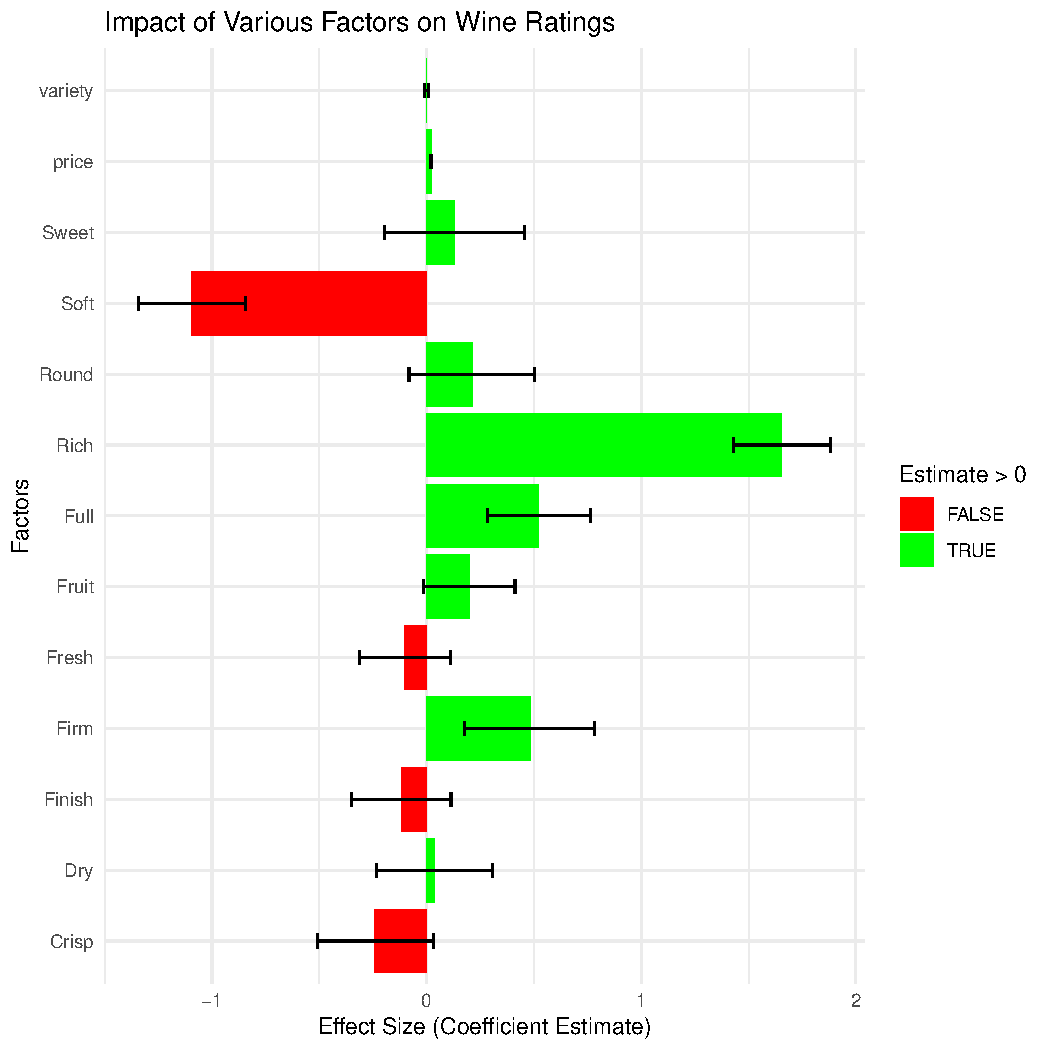
\includegraphics[width=0.5\textwidth]{imgs/Impact_box.pdf}
	\caption{Impact of Various Factors on Wine Ratings}
	\label{fig:impacts}
\end{figure}

Key insight from this paper is shown in Figure \ref{fig:impacts}. The analysis revealed that specific sensory attributes such as 'Rich', 'Full', and 'Firm' positively correlate with higher wine ratings, suggesting that these are highly prized qualities in wine perception. Conversely, the 'Soft' attribute was consistently associated with lower ratings. Interestingly, although there is a positive correlation between price and points, variety does not have a significant effect on points, which means that other factors are more influential.

In conclusion, this paper investigate the factors affecting wine points and attempts to summarise the interrelationships of the factors by using statistical modelling. This paper can provide some reference for the quality and marketing of French wines in some aspects, and can also be used as an example for other similar studies.

The code used in this paper can be found at \href{https://github.com/cky008/wine-analysis}{GitHub(https://github.com/cky008/wine-analysis)}.


\section{Introduction}

Wine is one of the most popular alcoholics worldwide. It has a rich history and cultural influence. Driven by increasing demand from both traditional and emerging markets, the global wine market has grown steadily\cite{belaj2022social}. Wine quality is determined by a complex interplay of factors, including grape variety, growing conditions, winemaking techniques, and aging processes, etc. Wine quality would be accepted by multiple factors, such as variety, growing conditions, winemaking techniques, aging processes, etc. Polyphenols, a diverse family of plant-derived compounds, have been found very important in recent research from \cite{gutierrez2021wine}. It’s said that it can influence both the sensory properties and potential health benefits of wine. Thus, understanding the relationship between those factors which will influence the quality of wine is very important for both producers and consumers.

So, based on the above paragraph, it's decided that the main objective of this study is to explore the factors influencing wine quality and ratings(points). And in this study we will use a dataset which has 2,500 French wine reviews adapted from \href{https://www.kaggle.com/datasets/zynicide/wine-reviews}{Kaggle}. The dataset includes information on key variables such as price, variety, Crisp, Dry, Finish, etc. and points(ratings), etc. In this dataset, wines rated $\geq 90$ would be considered as "superior"($superio\_rating = 1$).

By applying statistical modeling techniques to this dataset, we gonna try to find the key factors of wine quality. And we also will try to develop a useful predictive models for estimating wine points based on those factors. The result may be helpful for production and marketing strategies for winemakers, or may be helpfule for decision-making for consumer, and also may be contribute to the broader understanding of wine as a product with deep connections to place, culture, and sensory experience.

The remainder of this paper is structured as follows: Section \ref{sec:execsummary} provides an executive summary and objective statement, followed by a central figure. Section \ref{sec:data} describes the wine review dataset and variables. Section \ref{sec:analysis} presents the statistical analysis and results. Finally, Section \ref{sec:conclusion} concludes by summarizing the main findings, evaluating the success of the methods, and offering recommendations for future research.

\section{Data Description}\label{sec:data}
The dataset from \href{https://www.kaggle.com/datasets/zynicide/wine-reviews}{Kaggle} to be analyzed includes the following variables:

\begin{itemize}
    \item \textbf{points}: The wine rating on a scale of 80-100 points, with wines rated $\$geq 90$ considered "superior".
    \item \textbf{superior\_rating}: A binary indicator of whether the wine is rated as "superior" (1) or not (0).
    \item \textbf{price}: The price of the wine in US dollars.
    \item \textbf{variety}: The grape variety used to produce the wine.
    \item \textbf{Crisp, Dry, Finish, Firm, Fresh, Fruit, Full, Rich, Round, Soft, Sweet}: Binary variables indicating the presence (1) or absence (0) of specific sensory attributes in the wine.
    \item \textbf{description}: A text variable containing the full review description for each wine.
\end{itemize}

To explore the relationships between variables, several visualizations were ploted in R. Figure \ref{fig:price_points} is a scatterplot where we can observe that there seems to be a positive correlation between the price of a wine and its rating on a 100-point scale. Most of the points are centred under \$200, with a wide range of ratings from 80 to 100. We can't draw too many concrete conclusions from this chart. But we can probably guess that the higher the price, the better the quality of the wine.
\begin{figure}[htbp]
	\centering
	\begin{minipage}{0.45\textwidth}
	\centering
	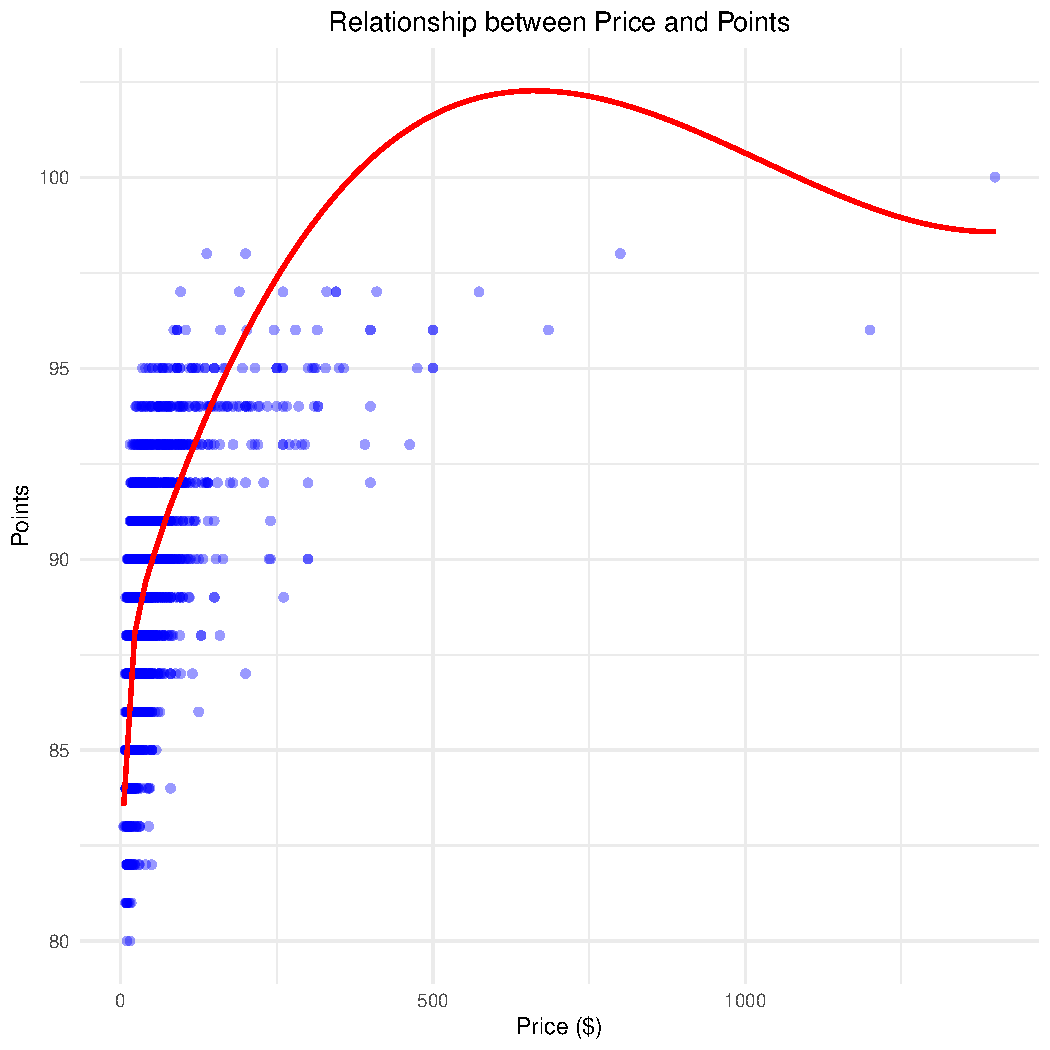
\includegraphics[width=\textwidth]{imgs/price_points_1.pdf}
	\caption{Relationship between Price and Points}
	\label{fig:price_points}
	\end{minipage}
	\hfill
	\begin{minipage}{0.45\textwidth}
	\centering
	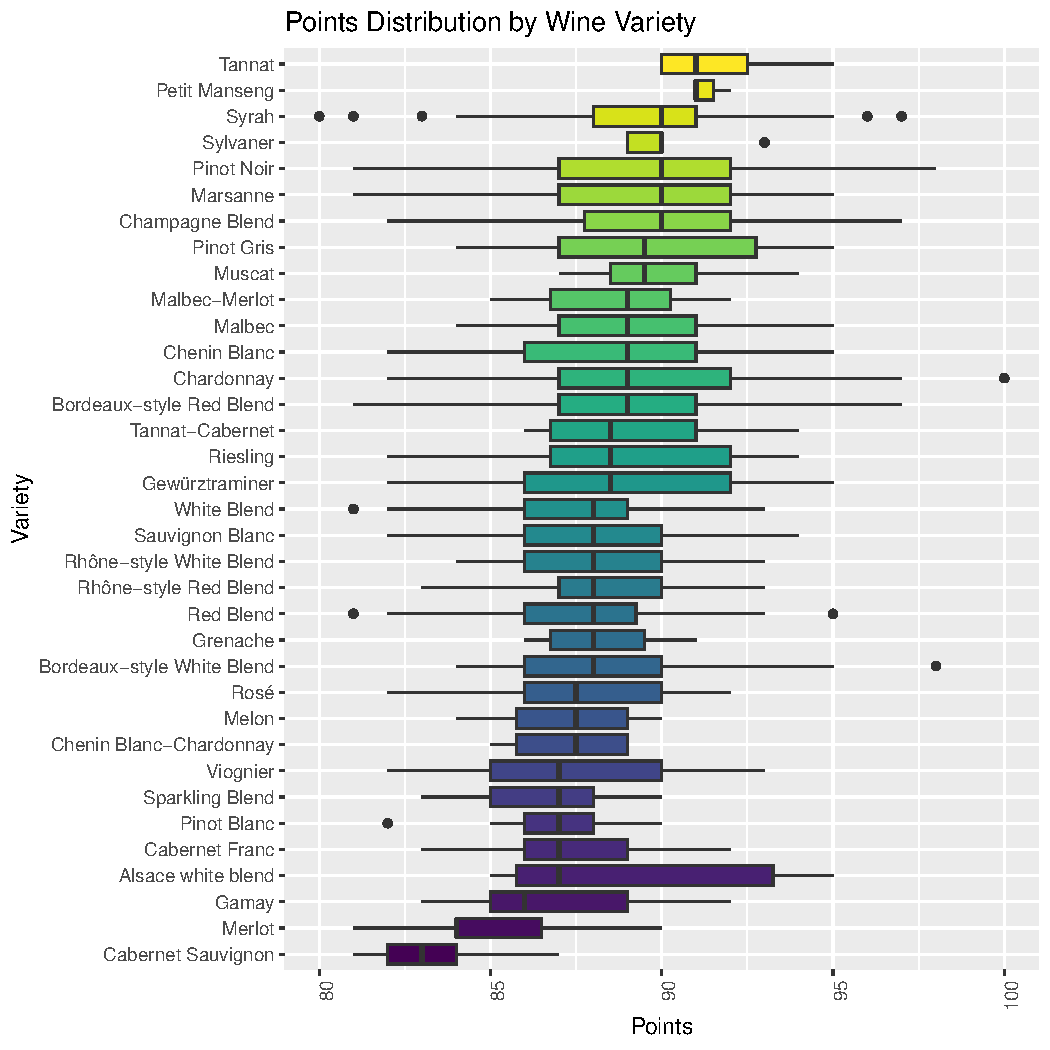
\includegraphics[width=\textwidth]{imgs/points_variety_1.pdf}
	\caption{Points Distribution by Wine Variety}
	\label{fig:points_variety}
	\end{minipage}
\end{figure}
	


The distribution of points across different wine varieties is plotted in Figure \ref{fig:points_variety}. As shown in Figure \ref{fig:points_variety}, the point distributions vary significantly across wine varieties. Like Tannat and Petit Manseng, they consistently receive high points, while others such as Cabernet Sauvignon and Merlot tend to have lower point. Many varieties show a wide range in their point distributions which showing there variable quality, while a few have tighter ranges which means that they more consistent qualities. 



To visualize the relationship between variety and the binary superior\_rating variable, a mosaic plot was plotted as Figure \ref{fig:variety_superior}. The plot indicates that certain varieties, such as Pinot Noir and Champagne Blend, have a higher proportion of wines rated as "superior" compared to others.
\begin{figure}[htbp]
	\centering
	\begin{minipage}{0.45\textwidth}
	\centering
	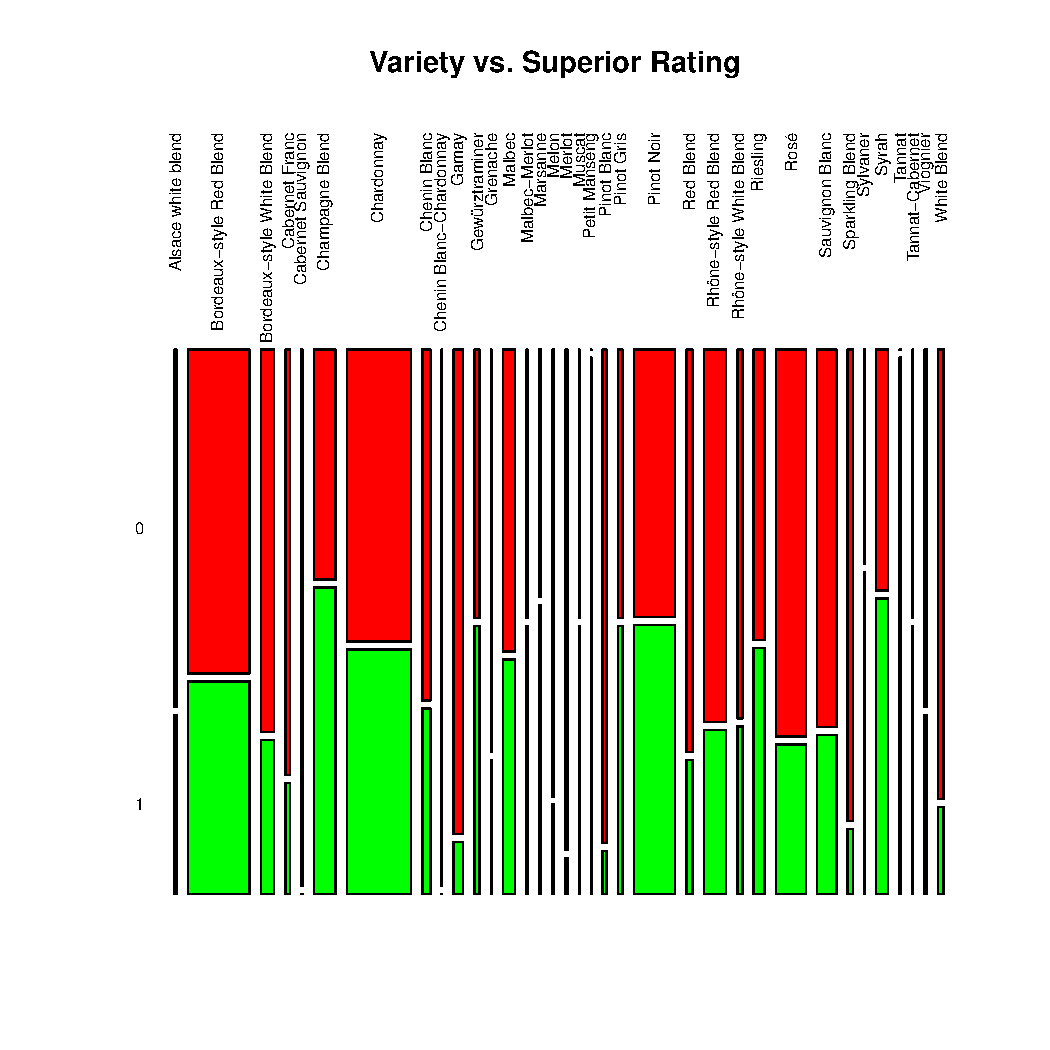
\includegraphics[width=\textwidth]{imgs/variety_superior.pdf}
	\caption{Variety vs. Superior Rating}
	\label{fig:variety_superior}
	\end{minipage}
	\hfill
	\begin{minipage}{0.45\textwidth}
	\centering
	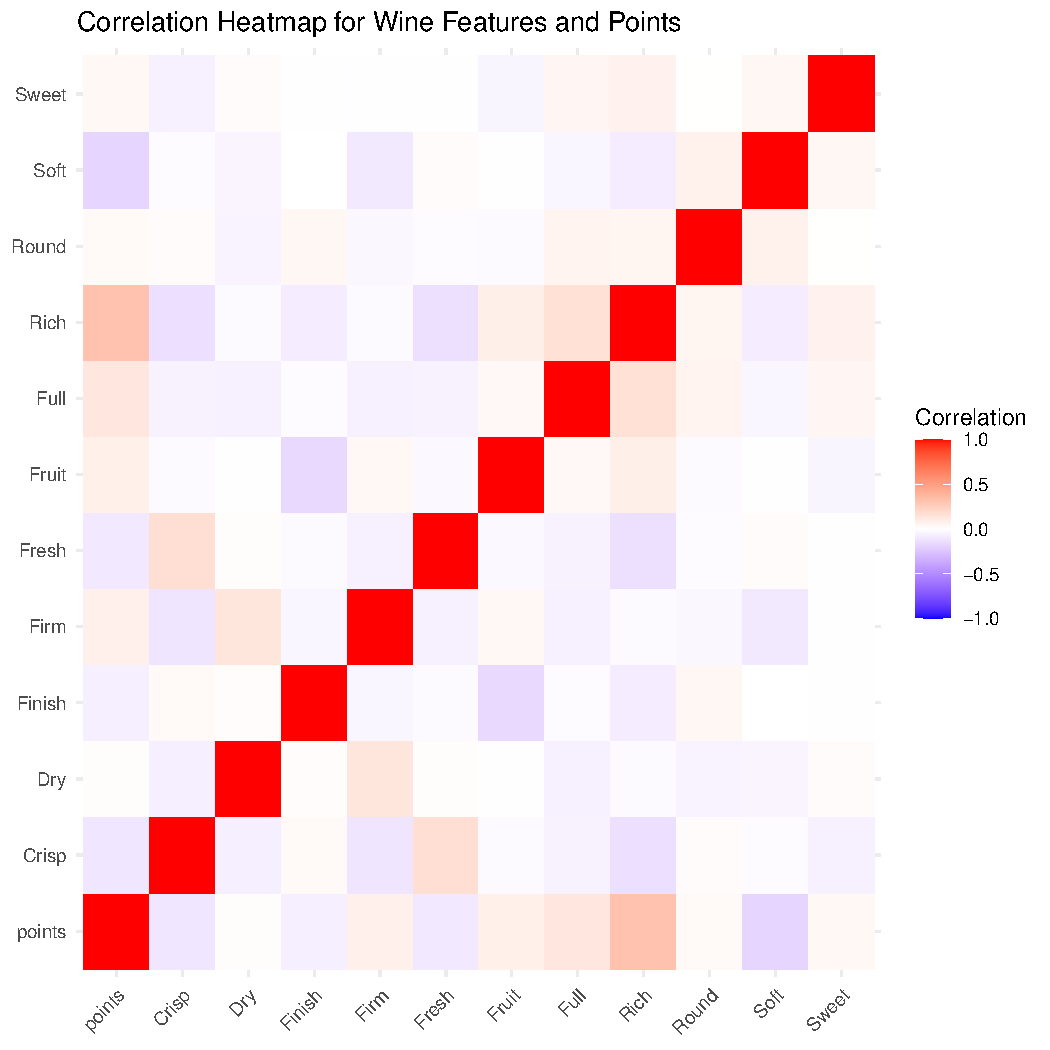
\includegraphics[width=\textwidth]{imgs/corr_heatmap.pdf}
	\caption{Correlation Heatmap for Wine Features and Points}
	\label{fig:corr_heatmap}
	\end{minipage}
\end{figure}

With the following code we can calculate the correlation matrix for the specified column of wine\_data.
\begin{verbatim}
	cor_matrix <- cor(wine_data[, c("points", "Crisp", "Dry", "Finish", 
	"Firm", "Fresh", "Fruit", "Full", "Rich", "Round", "Soft", "Sweet")])
\end{verbatim}
Based on the result, the correlations heatmap for points and the binary sensory attributes such as Crisp, Dry, Finish, etc. was plotted in Figure \ref{fig:corr_heatmap}. From this graph it is easy to see that Rich and Soft have a greater influence on points.

These exploratory analyses provide valuable insights into the relationships between wine characteristics and quality ratings, setting the stage for the development of predictive models in the subsequent sections.
\section{Analysis}\label{sec:analysis}
\subsection{Modeling Approach}
The Bayesian linear regression method has advantages in incorporating prior knowledge and dealing with complex relationships in the data. This method allows the integration of a priori beliefs about the parameters. This is particularly useful in the context of our research direction (wine points). In addition, this approach provides a probabilistic framework, which allows us to estimate and predict uncertainty in a more comprehensive way. 

This is ideal for dealing with the nuances of wine quality assessment. In Figure \ref{fig:corr_heatmap} we can see that the various elements interact with each other, influence each other and they combine to affect the points of the wines. It is for this reason that by using Bayesian Linear Regression we can make more informed predictions.

The final model used to predicts the points rating is based on price, variety(The variety is mapping to numbers for the models.), and the 12 binary sensory attributes:
\begin{equation*}
	\text{points} \sim \text{price} + \text{variety} + \text{Crisp} + \text{Dry} + \text{Finish} + \text{Firm} + \text{Fresh} + \text{Fruit} + \text{Full} + \text{Rich} + \text{Round} + \text{Soft} + \text{Sweet}
\end{equation*}

The model was implemented using the \texttt{brms} package in R, with the following priors:
\begin{itemize}
\item Normal(0, 10) prior for the regression coefficients
\item Normal(88, 3) prior for the intercept
\end{itemize}

The model was fit using 4 chains, each with 2000 iterations (500 warmup). The key code for fitting the model is shown below:
\begin{lstlisting}
	model <- brm(points ~ price + variety + Crisp + Dry + Finish + Firm + Fresh + Fruit + Full + Rich + Round + Soft + Sweet,
	data = wine_data,
	family = gaussian(), 
	prior = c(set_prior("normal(0, 10)", class = "b"), 
						set_prior("normal(88, 3)", class = "Intercept")),
	chains = 4, iter = 2000, warmup = 500,
	control = list(adapt_delta = 0.95))
\end{lstlisting}

\subsection{Model Results}
\begin{table}[htbp]
	\centering
	\caption{Bayesian linear regression model summary}
	\label{tab:model_summary}
\begin{tabular}{lccccccc}
	\toprule
	\textbf{Variable} & \textbf{Estimate} & \textbf{Est.Error} & \textbf{l-95\% CI} & \textbf{u-95\% CI} & \textbf{Rhat} & \textbf{Bulk\_ESS} & \textbf{Tail\_ESS} \\
	\midrule
	Intercept & 87.09 & 0.15 & 86.79 & 87.38 & 1.00 & 9092 & 4396 \\
	price     & 0.02  & 0.00 & 0.02  & 0.02  & 1.00 & 6123 & 3751 \\
	variety   & 0.00  & 0.00 & -0.01 & 0.01  & 1.00 & 13120 & 4344 \\
	Crisp     & -0.24 & 0.14 & -0.51 & 0.03  & 1.00 & 8895 & 4538 \\
	Dry       & 0.04  & 0.14 & -0.23 & 0.31  & 1.00 & 8510 & 4316 \\
	Finish    & -0.12 & 0.12 & -0.35 & 0.11  & 1.00 & 8599 & 5125 \\
	Firm      & 0.48  & 0.16 & 0.18  & 0.78  & 1.00 & 6898 & 4683 \\
	Fresh     & -0.10 & 0.11 & -0.31 & 0.11  & 1.00 & 8105 & 4661 \\
	Fruit     & 0.20  & 0.11 & -0.01 & 0.41  & 1.00 & 9562 & 4625 \\
	Full      & 0.52  & 0.12 & 0.28  & 0.76  & 1.00 & 8157 & 4407 \\
	Rich      & 1.65  & 0.11 & 1.43  & 1.88  & 1.00 & 7052 & 4792 \\
	Round     & 0.21  & 0.15 & -0.08 & 0.50  & 1.00 & 8615 & 4911 \\
	Soft      & -1.09 & 0.13 & -1.34 & -0.84 & 1.00 & 8208 & 4525 \\
	Sweet     & 0.13  & 0.17 & -0.20 & 0.46  & 1.00 & 10375 & 4433 \\
	\midrule
	$\sigma$ & 2.45 & 0.03 & 2.38 & 2.52 & 1.00 & 9998 & 4354 \\
	\bottomrule
\end{tabular}
\end{table}

The model summary which showed in Table \ref{tab:model_summary} shows several significant predictors of wine ratings. The intercept estimate of 87.09 indicates that, when all other variables are zero, the predicted wine rating is 87.09 points. The price coefficient of 0.02 suggests that, holding other variables constant, a one-dollar increase in price is associated with a 0.02-point increase in the predicted wine rating. The variety coefficient is close to zero, implying that the variety has a minimal impact on the rating.

Several sensory attributes have significant effects on the wine ratings. The Rich attribute has a large positive coefficient of 1.65, indicating that wines with this attribute tend to receive substantially higher ratings. In contrast, the Soft attribute has a large negative coefficient of -1.09, suggesting that wines with this attribute are likely to receive lower ratings. The Full and Firm attributes also have positive coefficients of 0.52 and 0.48, respectively, implying that these attributes contribute to higher wine ratings. The Crisp attribute has a small negative coefficient of -0.24, indicating a slight negative impact on the rating.

The Rhat values are all equal to 1, indicating good convergence of the MCMC sampling. The large Bulk\_ESS and Tail\_ESS values suggest that the effective sample sizes are sufficient, and the model estimates are reliable. The residual standard deviation ($\sigma$) is estimated to be 2.45, reflecting the random error in the predictions.

Overall, Table \ref{tab:model_summary} provides rich information about the factors influencing wine ratings and confirms the reliability of the model fit. Price and sensory attributes such as Rich, Full, and Firm have positive effects on the ratings, while the Soft attribute has a negative impact. These findings can help understand the key drivers of wine quality perceptions and guide the development of targeted marketing strategies.


The Figure \ref{fig:combined_predictors} display the posterior distributions of coefficients in the Bayesian linear regression model. From these plots, we can observe that most parameters exhibit reasonable shapes and locations in their posterior distributions. The intercept term concentrates its posterior mass in the high-value range between 86.5 and 87.5. The coefficients for price, variety, and most taste features have their posterior distributions primarily centered around 0, but with varying shapes and degrees of deviation from 0, indicating their differential impact on wine points. Overall, by examining the graphical posterior distributions, we gain insights into the role and importance of each variable in predicting wine points, and the plausible posterior shapes boost our confidence in the model fit quality.


\begin{figure}[htbp]
	\centering
	\begin{minipage}{0.45\textwidth}
		\centering
		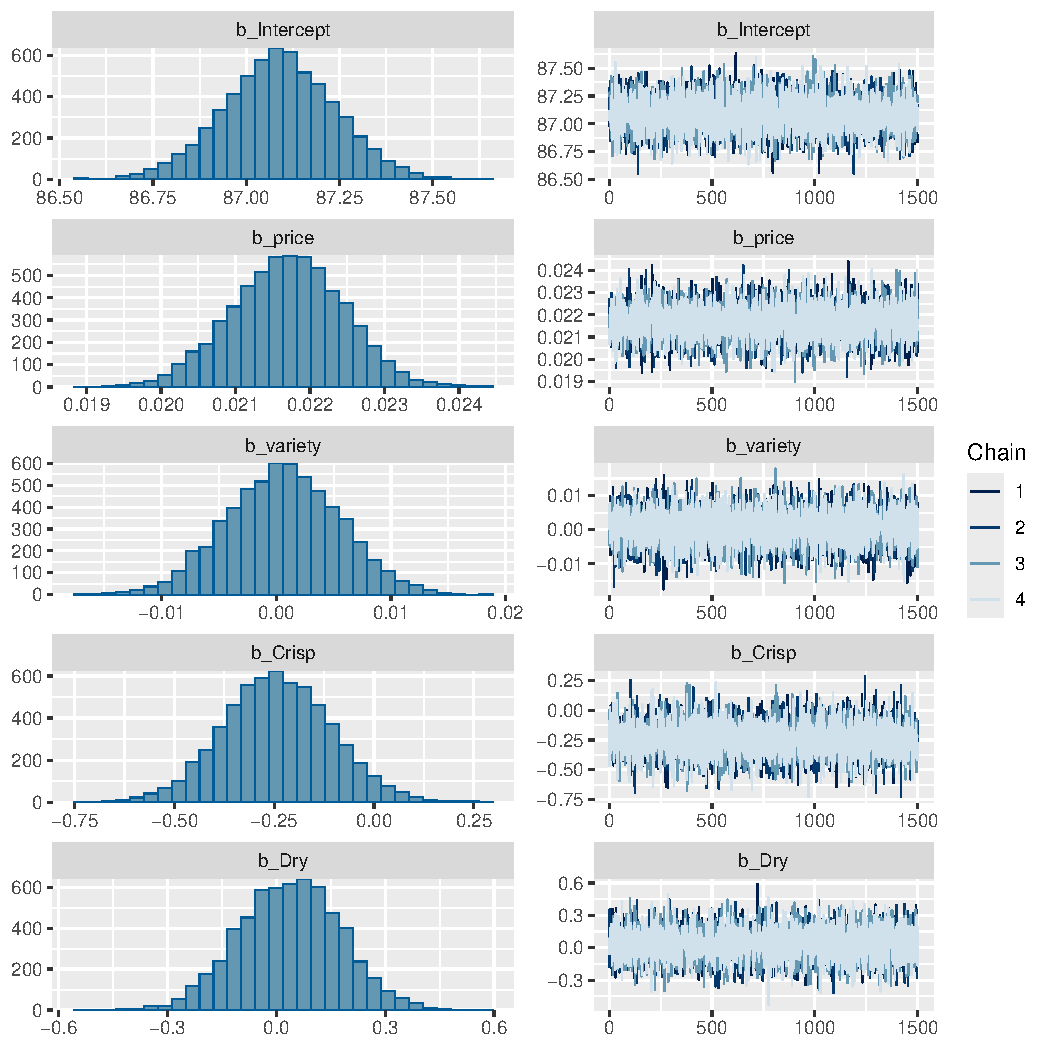
\includegraphics[width=\textwidth]{imgs/histograms_trace_plots_1.pdf}
	\end{minipage}
	\hfill
	\begin{minipage}{0.45\textwidth}
		\centering
		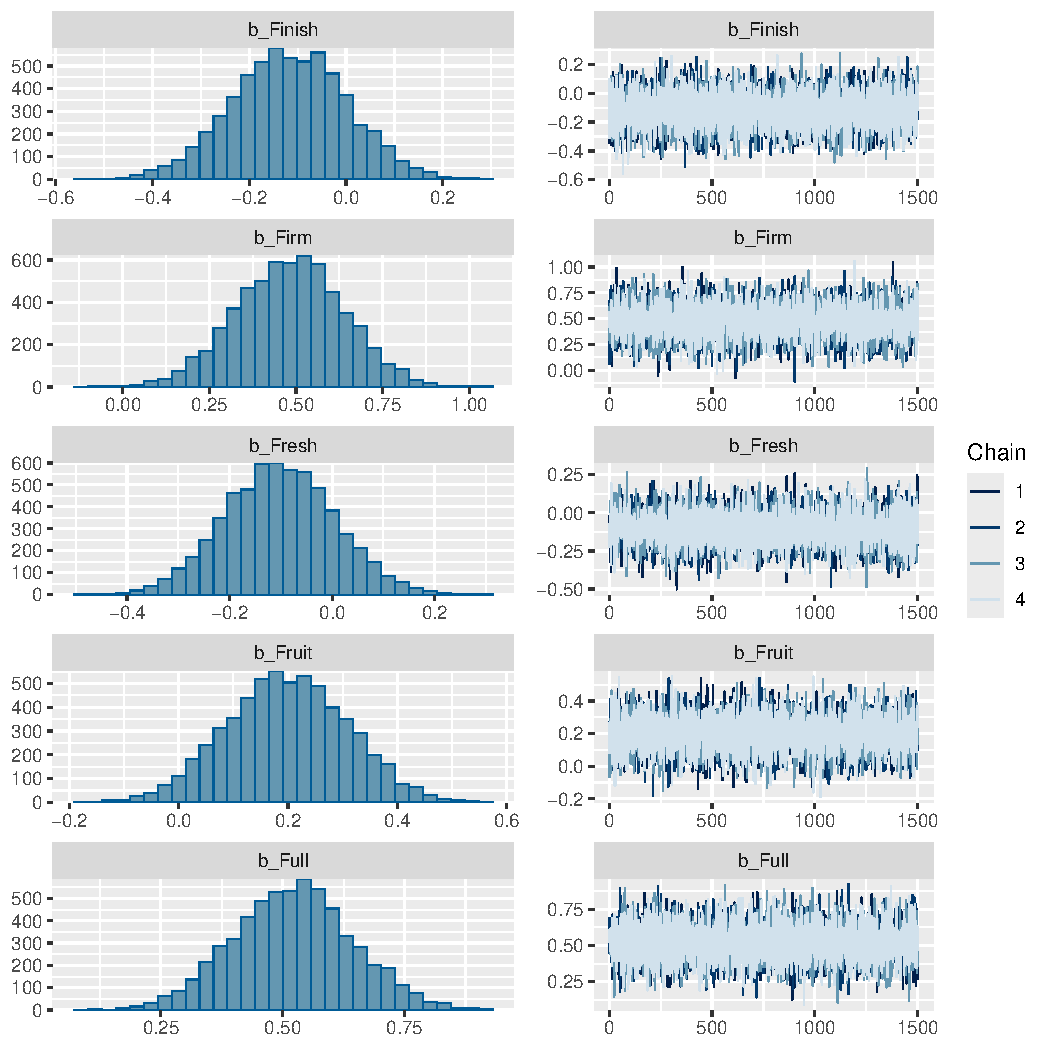
\includegraphics[width=\textwidth]{imgs/histograms_trace_plots_2.pdf}
	\end{minipage}
	\vspace{1cm} % This adds some vertical space before the third figure
	\begin{minipage}{0.45\textwidth}
		\centering
		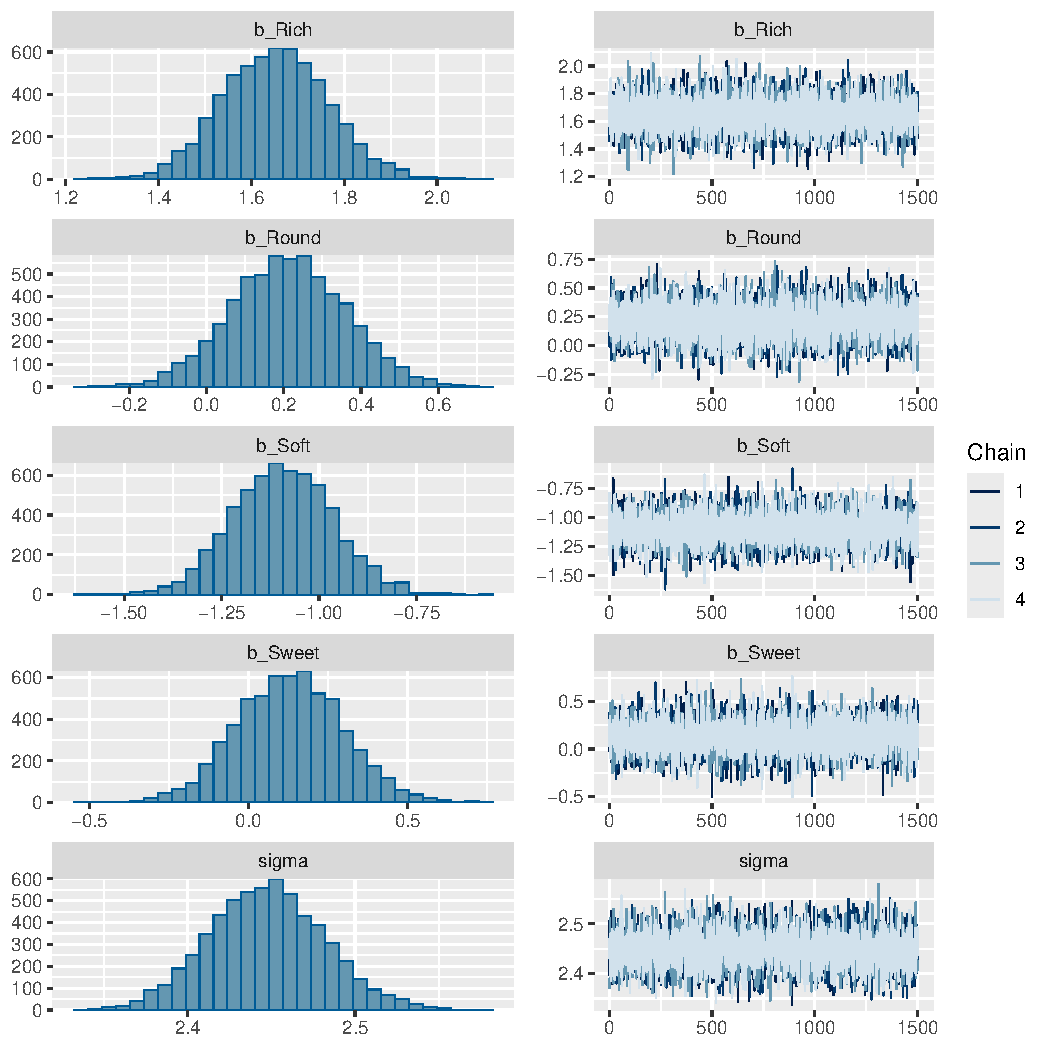
\includegraphics[width=\textwidth]{imgs/histograms_trace_plots_3.pdf}
	\end{minipage}
	\caption{Histograms and Trace Plots from Bayesian Linear Regression Model}
	\label{fig:combined_predictors}
\end{figure}


The Figure \ref{fig:conditional_effects} are conditional effects plots which show the relationships between various predictors and the wine ratings, controlling for other variables in the model. Each plot displays how changes in one specific predictor, such as price or descriptive attributes like "Firm" or "Rich", influence the wine's rating (points). The blue line represents the mean effect while the shaded area indicates the 95\% confidence interval, giving insight into the certainty of these effects. Notably, some attributes like "Rich" and "Full" show a positive effect on the ratings, increasing as the attribute value increases, while others like "Soft" exhibit a negative relationship, where higher values correlate with lower ratings. These figures help us to understand which factors have a greater influence on the quality of a wine.


% Figure \ref{fig:conditional_effects} shows the conditional effects relationships between various predictor variables and wine ratings, while controlling for other variables in the model. Each subplot demonstrates how changes in a specific predictor variable (such as price or descriptive attributes like "Firm" or "Rich") influence the wine's rating (points), holding other predictors constant at their mean values. The blue line represents the mean estimated effect, and the shaded area indicates the 95\% confidence interval of the estimated effects, reflecting the uncertainty in these effect estimates. Notably, some attributes like "Rich" and "Full" exhibit a positive effect on the ratings, increasing as the attribute value increases; while others like "Soft" show a negative relationship, where higher values are associated with lower ratings. Variables such as price and vintage appear to have a non-linear relationship with the wine rating. These visualizations are crucial for understanding which characteristics are most influential in determining the perceived quality of wines and highlight the subtle interplay among various wine features. However, they do not provide information about the overall predictive performance of the model or the relative importance of each variable.

\begin{figure}[htbp]
	\centering
	% 第一行图像
	\begin{subfigure}{0.22\textwidth}
		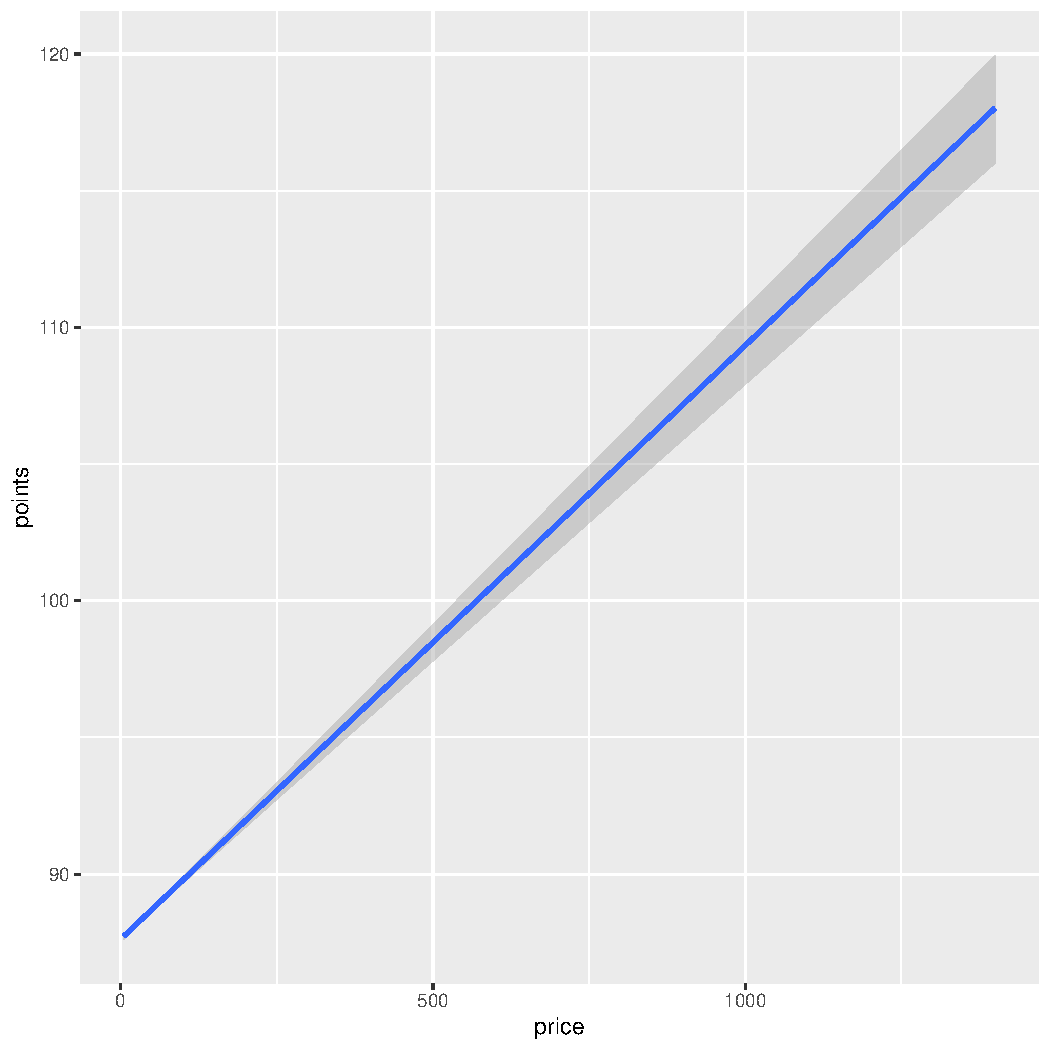
\includegraphics[width=\textwidth]{imgs/Rplots-11.pdf}
	\end{subfigure}\hfill
	\begin{subfigure}{0.22\textwidth}
		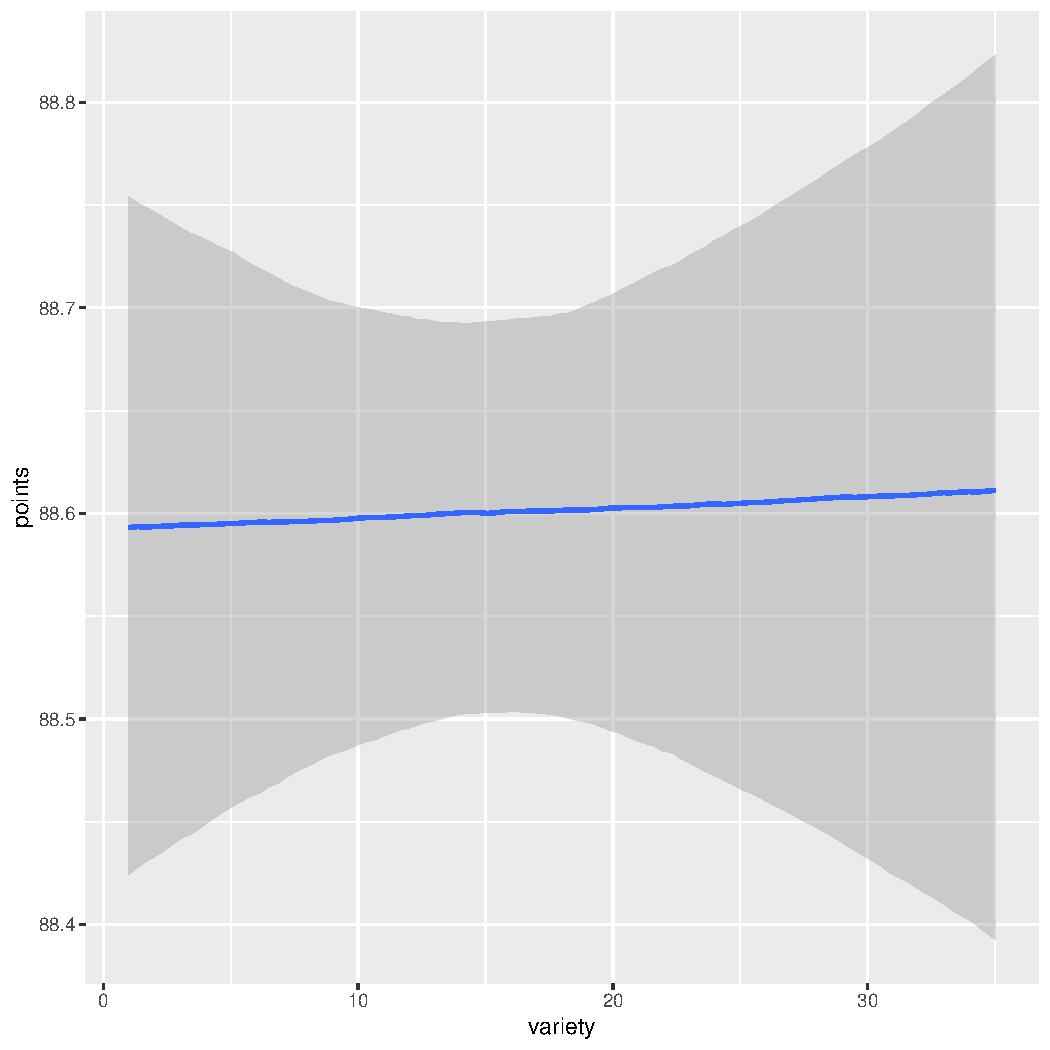
\includegraphics[width=\textwidth]{imgs/Rplots-12.pdf}
	\end{subfigure}\hfill
	\begin{subfigure}{0.22\textwidth}
		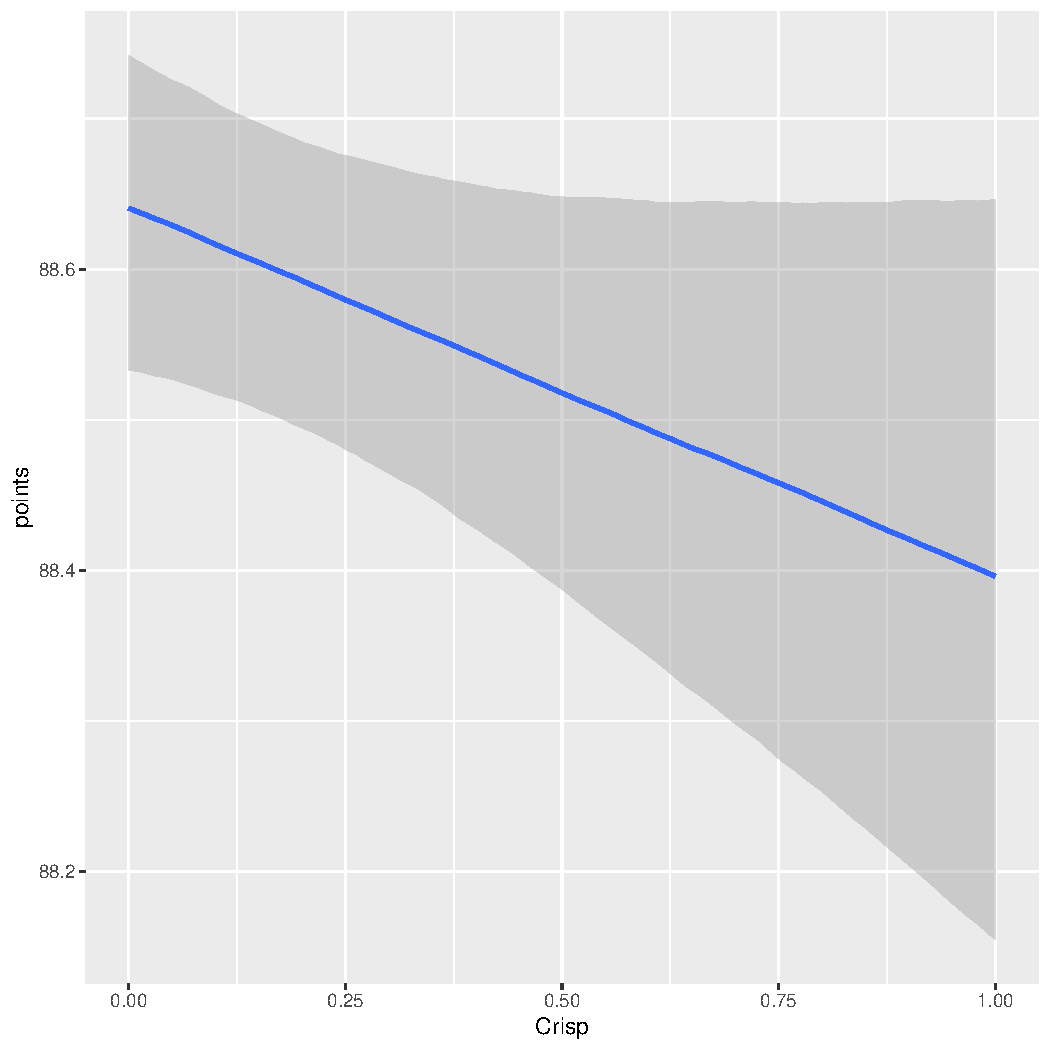
\includegraphics[width=\textwidth]{imgs/Rplots-13.pdf}
	\end{subfigure}\hfill
	\begin{subfigure}{0.22\textwidth}
		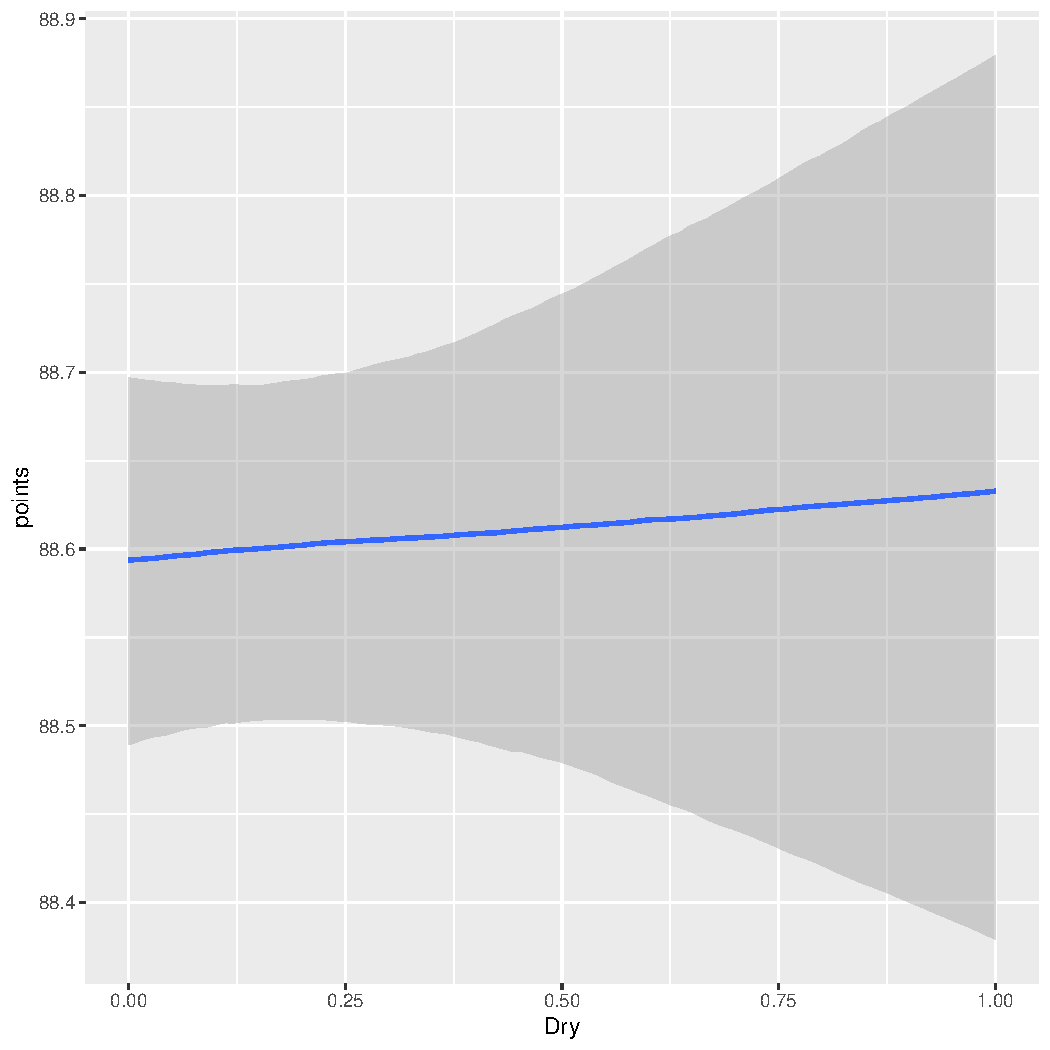
\includegraphics[width=\textwidth]{imgs/Rplots-14.pdf}
	\end{subfigure}
	
	% 第二行图像
	\begin{subfigure}{0.22\textwidth}
		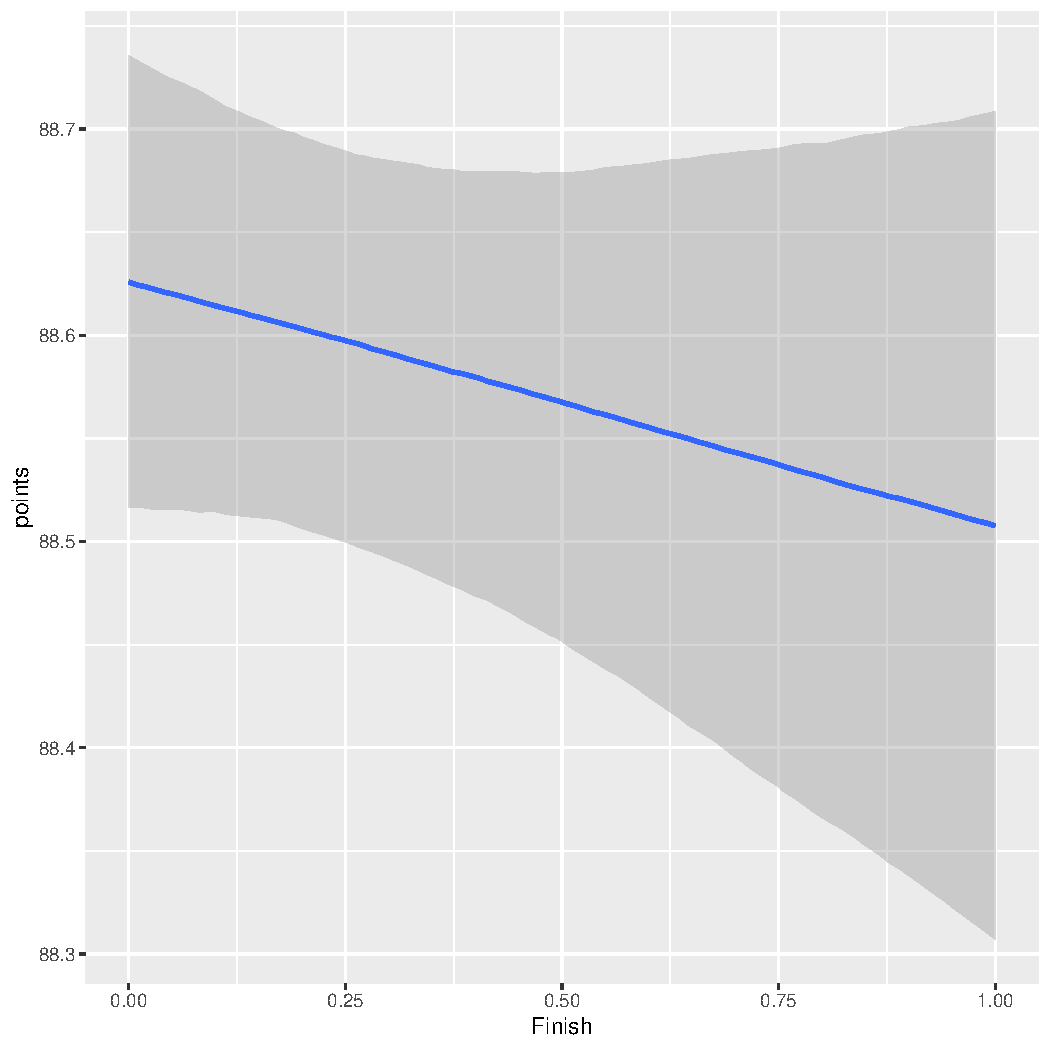
\includegraphics[width=\textwidth]{imgs/Rplots-15.pdf}
	\end{subfigure}\hfill
	\begin{subfigure}{0.22\textwidth}
		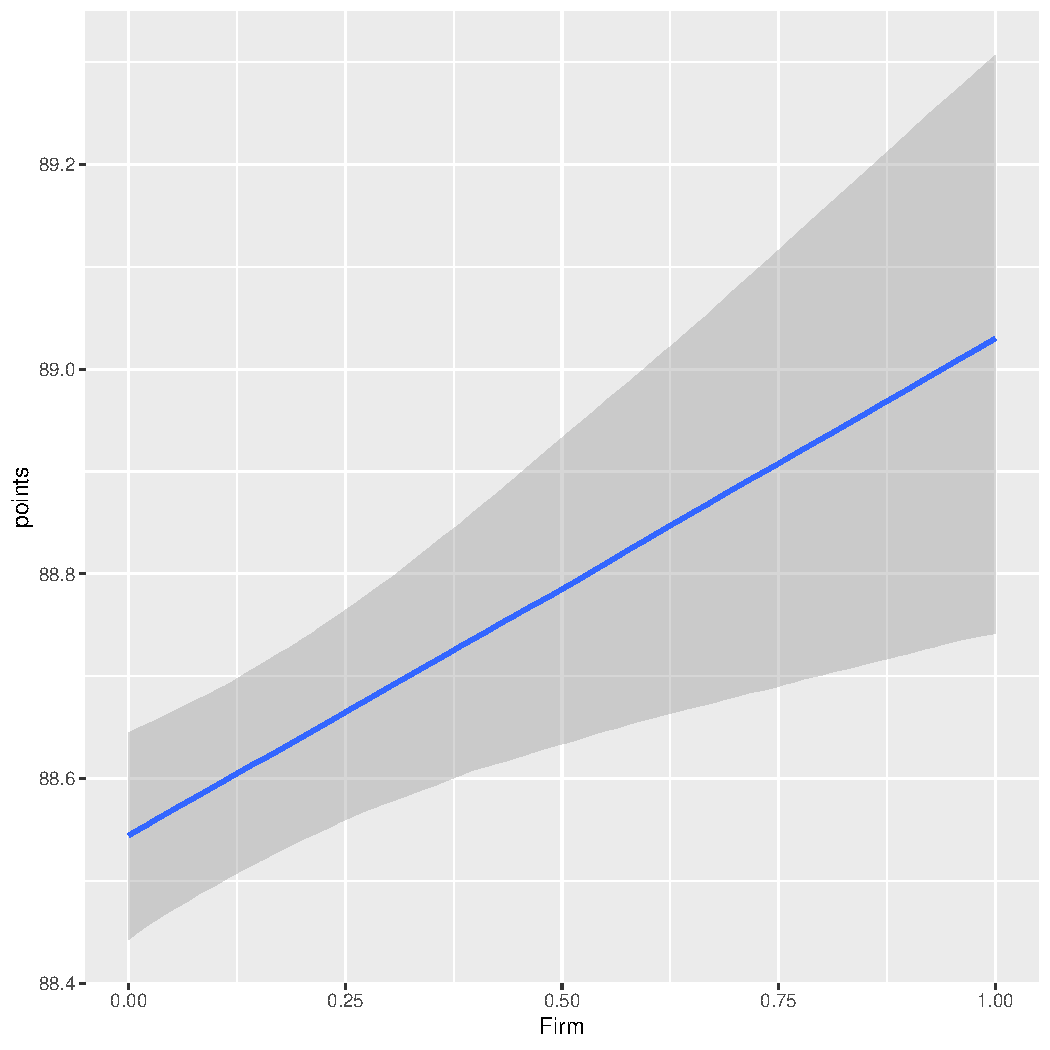
\includegraphics[width=\textwidth]{imgs/Rplots-16.pdf}
	\end{subfigure}\hfill
	\begin{subfigure}{0.22\textwidth}
		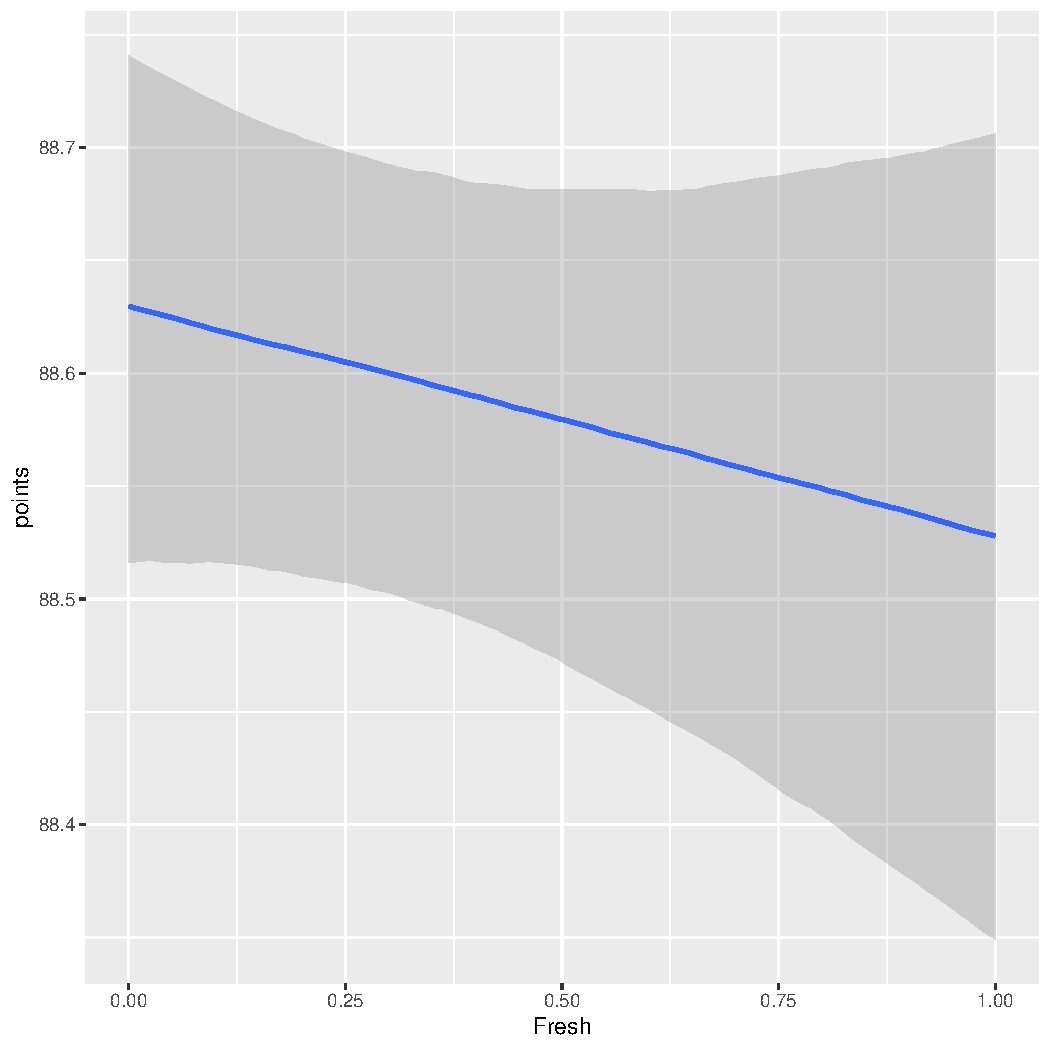
\includegraphics[width=\textwidth]{imgs/Rplots-17.pdf}
	\end{subfigure}\hfill
	\begin{subfigure}{0.22\textwidth}
		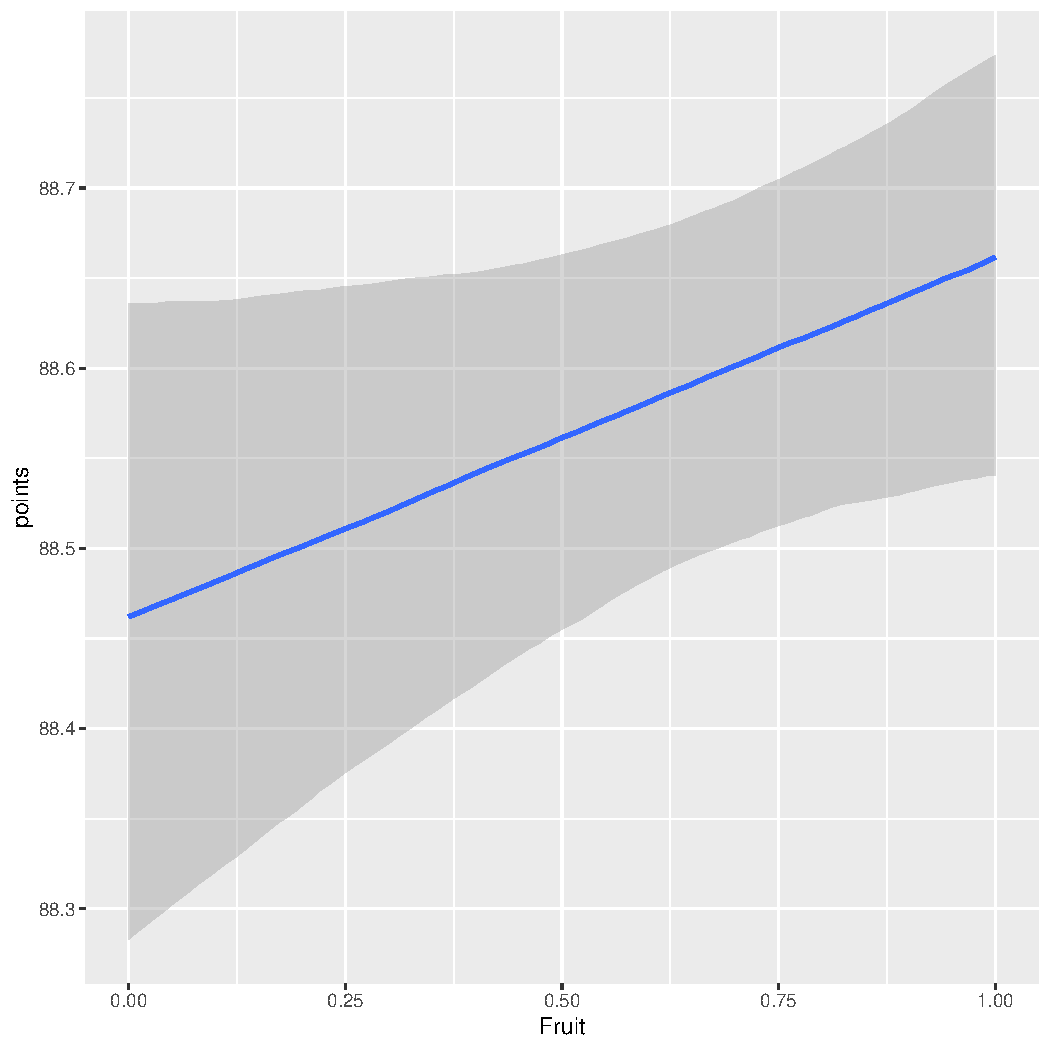
\includegraphics[width=\textwidth]{imgs/Rplots-18.pdf}
	\end{subfigure}
	
	% 第三行图像
	\begin{subfigure}{0.22\textwidth}
		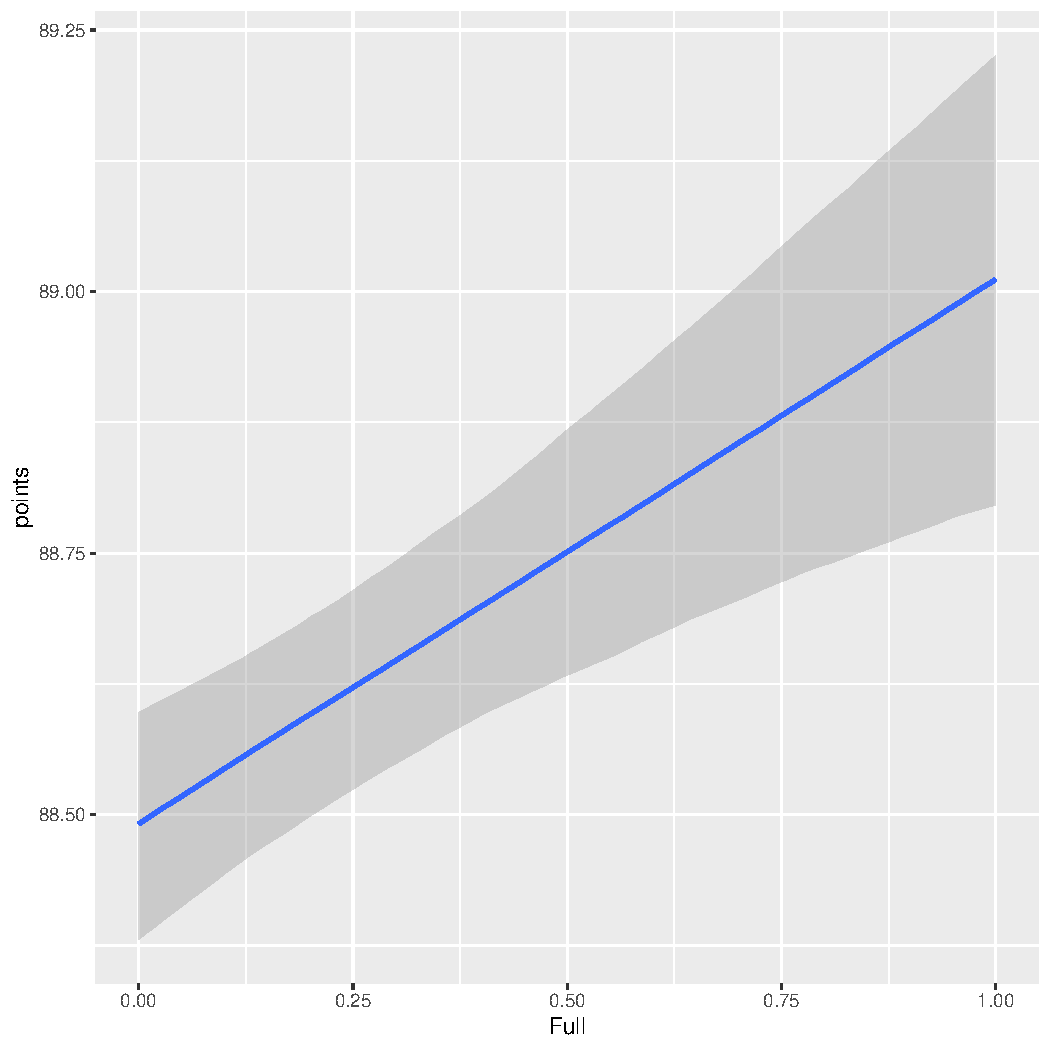
\includegraphics[width=\textwidth]{imgs/Rplots-19.pdf}
	\end{subfigure}\hfill
	\begin{subfigure}{0.22\textwidth}
		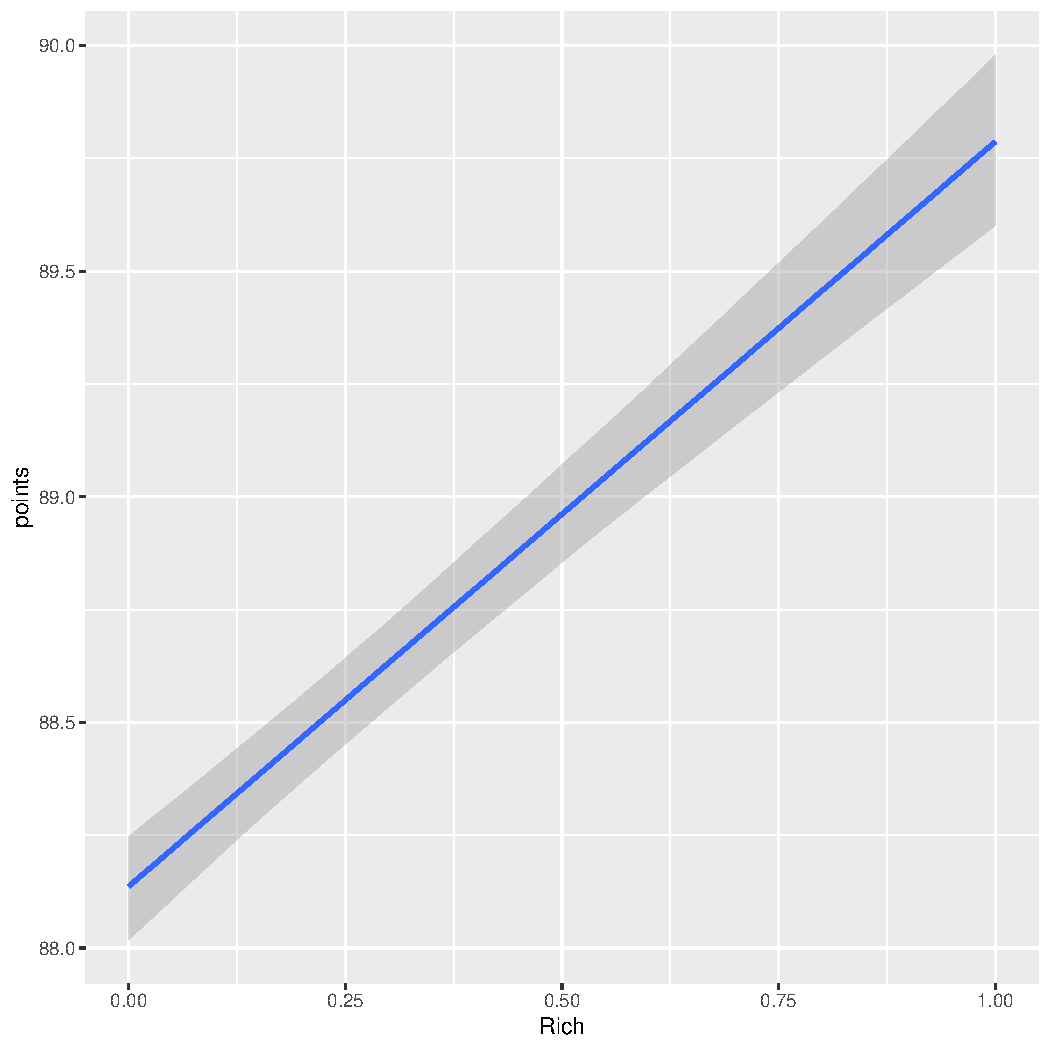
\includegraphics[width=\textwidth]{imgs/Rplots-20.pdf}
	\end{subfigure}\hfill
	\begin{subfigure}{0.22\textwidth}
		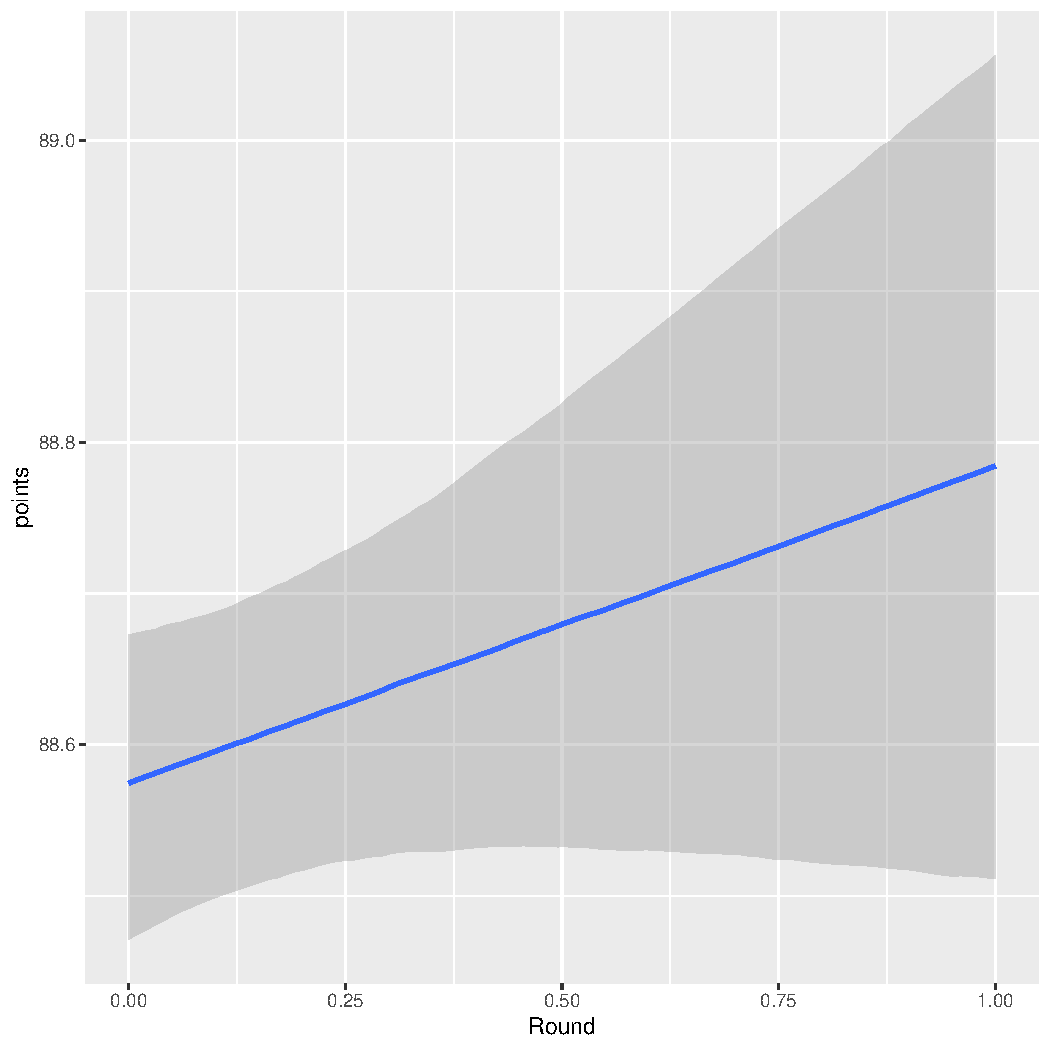
\includegraphics[width=\textwidth]{imgs/Rplots-21.pdf}
	\end{subfigure}\hfill
	\begin{subfigure}{0.22\textwidth}
		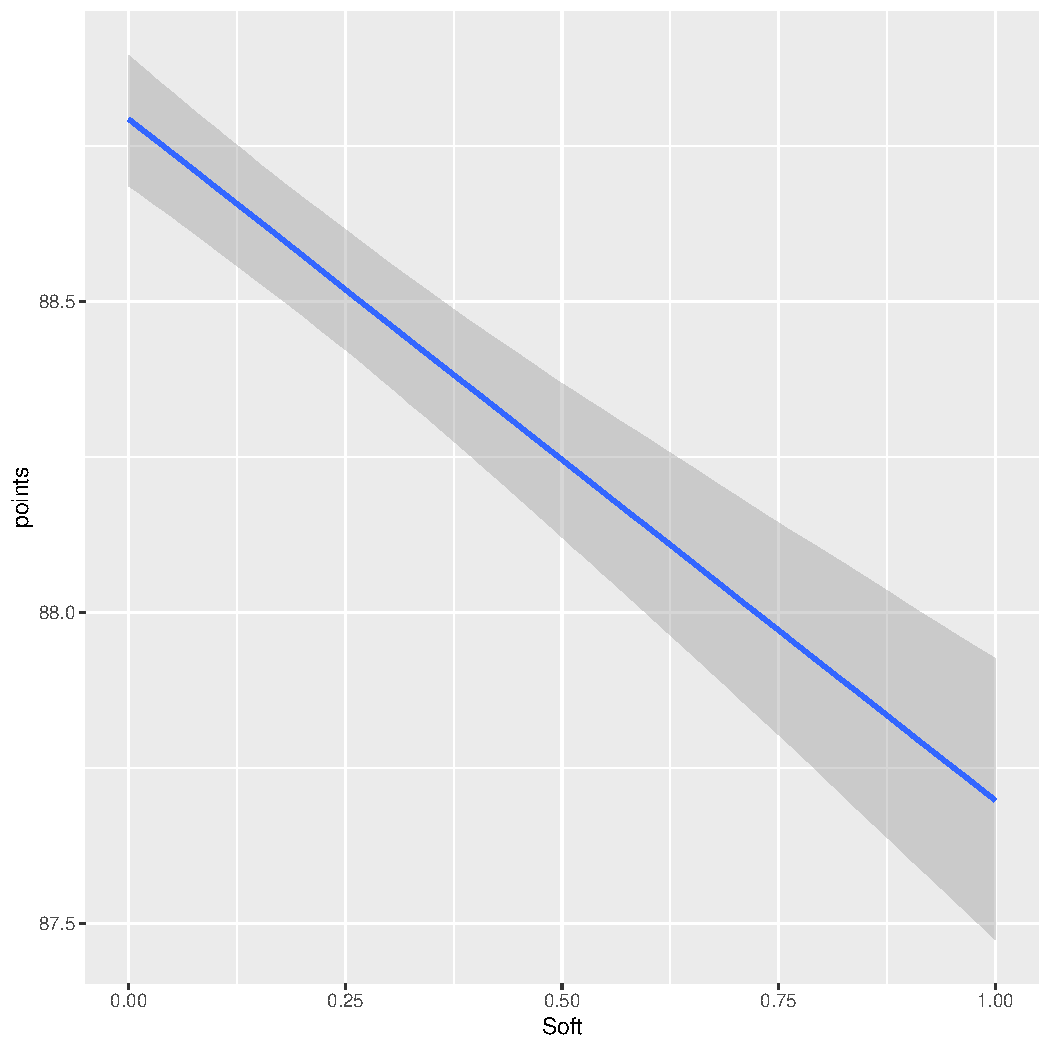
\includegraphics[width=\textwidth]{imgs/Rplots-22.pdf}
	\end{subfigure}
	
	% 第四行图像
	\begin{subfigure}{0.22\textwidth}
		\centering
		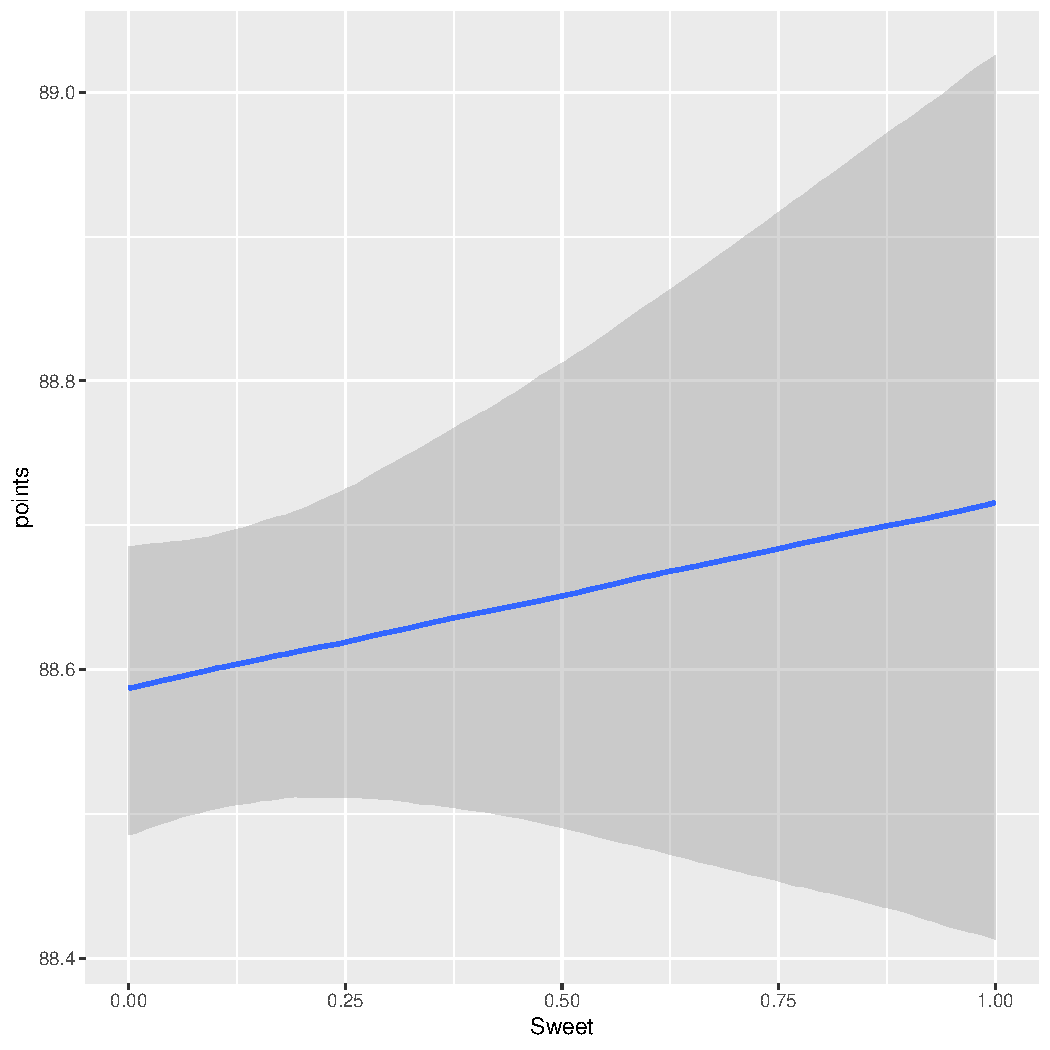
\includegraphics[width=\textwidth]{imgs/Rplots-23.pdf}
	\end{subfigure}
	
	\caption{Conditional Effects Plots from Bayesian Linear Regression Model}
	\label{fig:conditional_effects}
\end{figure}



% The Figure \ref{fig:Pairs_Scatter_Plots} is helpful for diagnosing the relationships among parameters in the Bayesian linear regression model. These pairs scatter plots reveal the distribution and correlation between each pair of parameters. Most notably, the plots do not show any clear linear relationships or distinct patterns such as funnel shapes or strong linear trends, which suggests that there is no severe multicollinearity between the parameters. This is a positive indication of the model's robustness, as it implies that each parameter contributes independently to the model without redundancy.

% Moreover, the circular and diffuse spread observed in most scatter plots indicates that the parameters are well-distributed and exhibit a reasonable degree of randomness, with no obvious signs of parameter constraints or unnatural bounds affecting the model. This kind of parameter interaction and independence is desirable in Bayesian modeling, ensuring that the posterior distributions are derived from a well-explored parameter space, enhancing the reliability and interpretability of the model's conclusions. Hence, the evidence from Figure \ref{fig:Pairs_Scatter_Plots} supports the model's structural integrity and suggests that the parameter estimates are stable and trustworthy.

Figure \ref{fig:Pairs_Scatter_Plots} is useful for understanding how the parameters in the Bayesian linear regression model relate to each other. ⁤⁤The pairs scatter plots show the spread and correlation between each pair of parameters. ⁤⁤Importantly, the plots don't reveal any obvious linear relationships or clear patterns like funnel shapes or strong linear trends. This suggests that there isn't serious multicollinearity between the parameters. ⁤⁤Multicollinearity means that parameters are too closely related, which can cause problems in the model. The lack of multicollinearity here is a good sign that the model is robust and that each parameter adds something unique to the model. ⁤
⁤In addition, most of the scatter plots show the parameters are spread out circularly and diffusely. This means the parameters are well-distributed and have a good amount of randomness. There are no clear signs that the parameters are being artificially limited or constrained. ⁤⁤This kind of parameter interaction and independence is good in Bayesian modelling. It ensures that the posterior distributions (the model's key results) are coming from a parameter space that has been thoroughly explored. This makes the model's conclusions more reliable and easier to interpret. ⁤⁤Therefore, the evidence from Figure \ref{fig:Pairs_Scatter_Plots} supports the overall structural integrity of the model. It suggests that the estimates of the parameters are stable and can be trusted. ⁤

\begin{figure}[htbp]
	\centering
	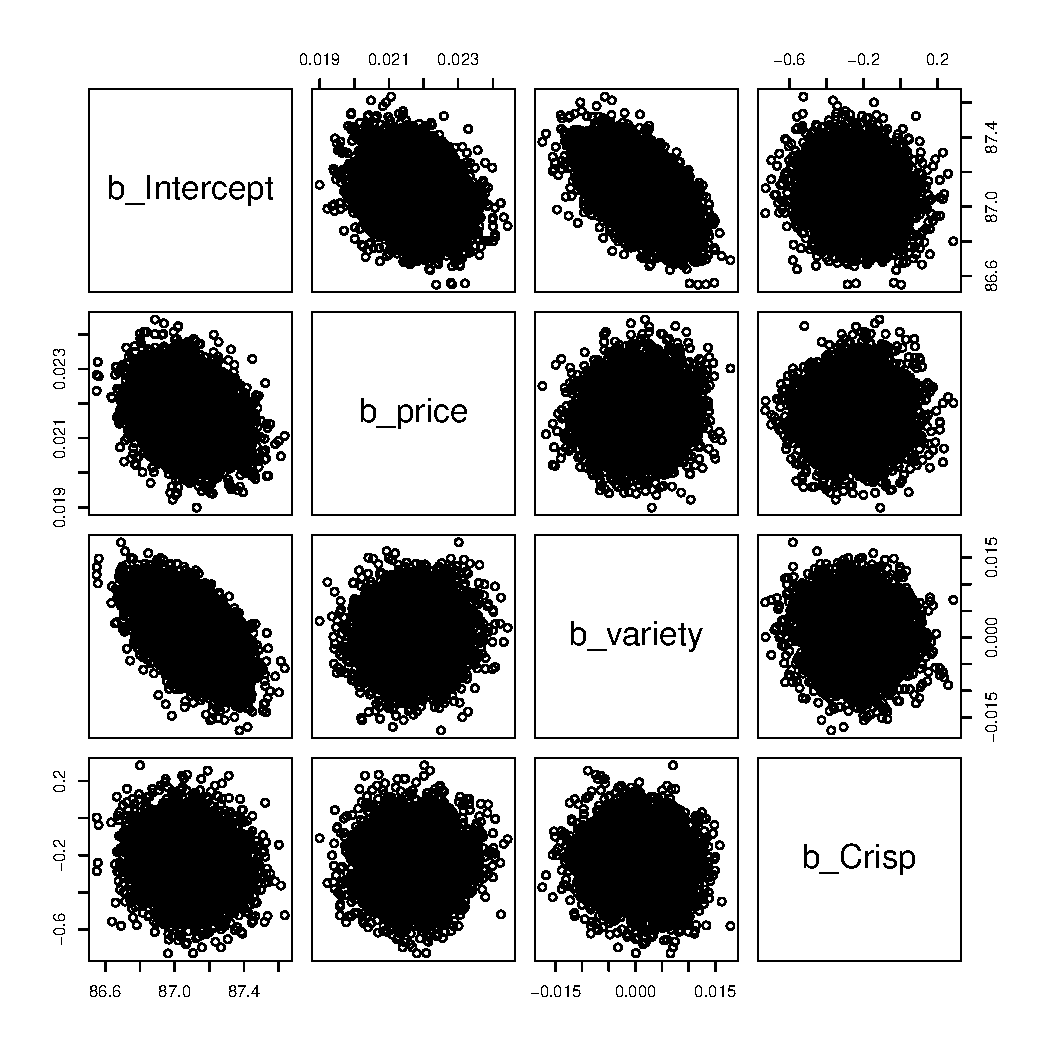
\includegraphics[width=0.6\textwidth]{imgs/Pairs_Scatter_Plots.pdf}
	\caption{Pairs Scatter Plots}
	\label{fig:Pairs_Scatter_Plots}
\end{figure}

Figures \ref{fig:a_v_p} and \ref{fig:a_v_p_2} present multiple visual assessments of the actual versus predicted points for wine quality points from a Bayesian linear regression model. These visualizations help evaluate the predictive accuracy of the model and identify areas for potential improvement.

The density and hexbin plots in Figure \ref{fig:a_v_p} show a general alignment along the diagonal, indicating a good fit between the predicted and actual points. However, deviations from this line, particularly in the density plot, suggest areas where the model's predictions diverge from actual values, especially in the mid-range points. The hexbin plot highlights regions of high and low prediction density, which helps pinpoint where the model performs well or poorly.

The actual vs. fitted plots with lines from Figure \ref{fig:a_v_p_2} further illustrate these points. The scatter plot reveals a spread of data around the diagonal, with some concentration near it but notable variability, especially at higher points. The actual vs. fitted plot connects predictions to actual values with lines, visually indicating prediction accuracy; shorter lines near the predicted axis show precise predictions, whereas longer lines indicate significant errors. These visual tools collectively demonstrate that while the model is generally effective, improvements could be targeted at reducing errors and enhancing prediction consistency across the point spectrum.

\begin{figure}[htbp]
	\centering
	% 三个图像在一行
	\begin{subfigure}{0.32\textwidth}
		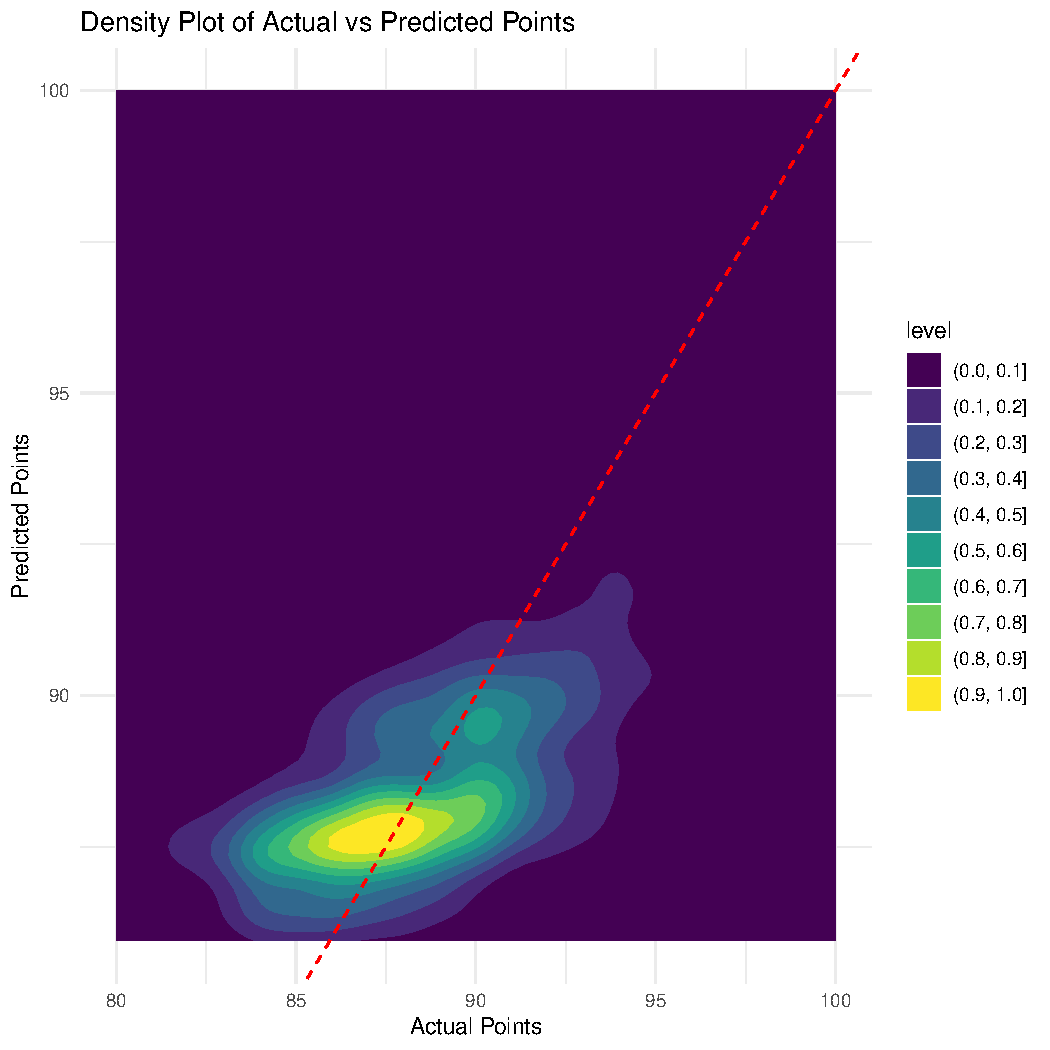
\includegraphics[width=\textwidth]{imgs/Rplots-29.pdf}
	\end{subfigure}\hfill
	\begin{subfigure}{0.32\textwidth}
		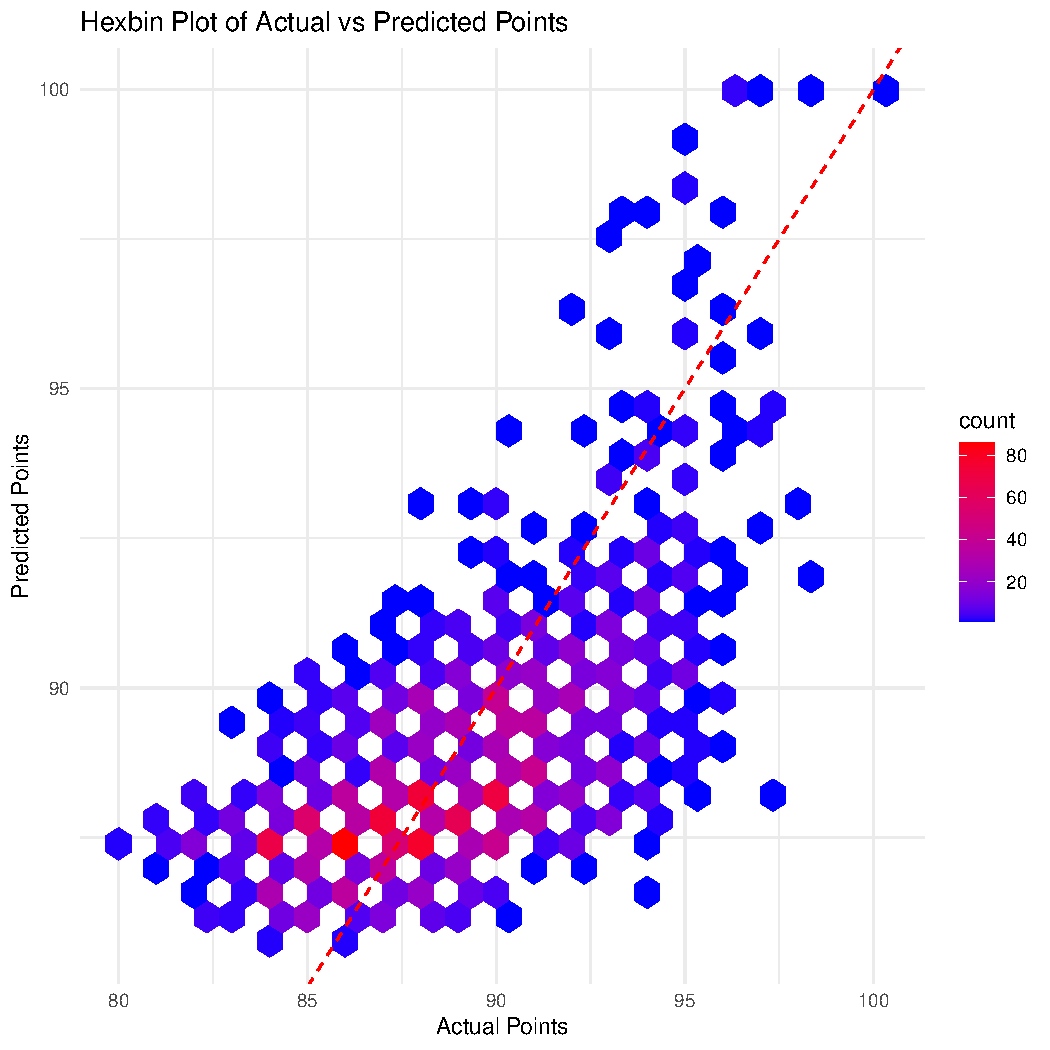
\includegraphics[width=\textwidth]{imgs/Rplots-28.pdf}
	\end{subfigure}\hfill
	\begin{subfigure}{0.32\textwidth}
		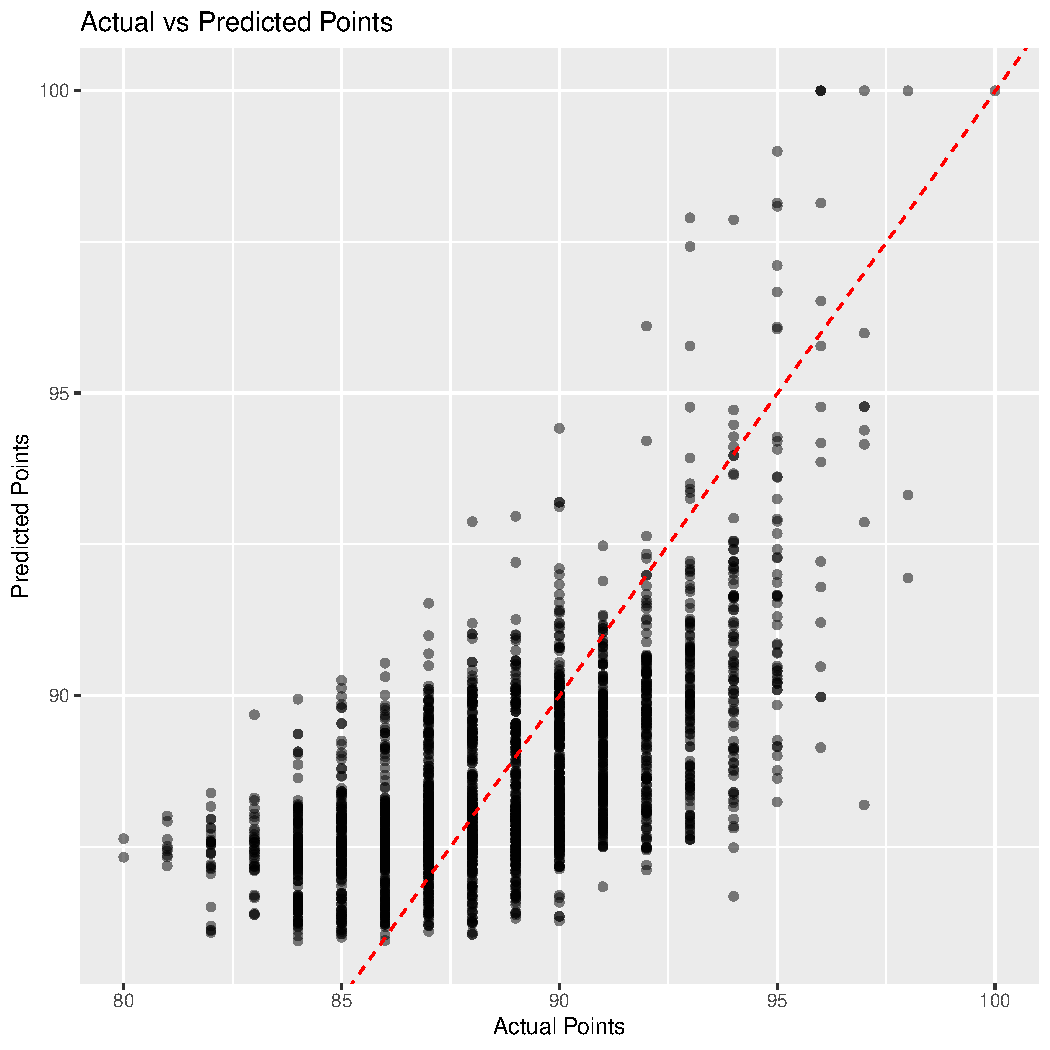
\includegraphics[width=\textwidth]{imgs/Rplots-26.pdf}
	\end{subfigure}
	
	\caption{Actual vs Predicted Points}
	\label{fig:a_v_p}
\end{figure}

\begin{figure}[htbp]
	\centering
	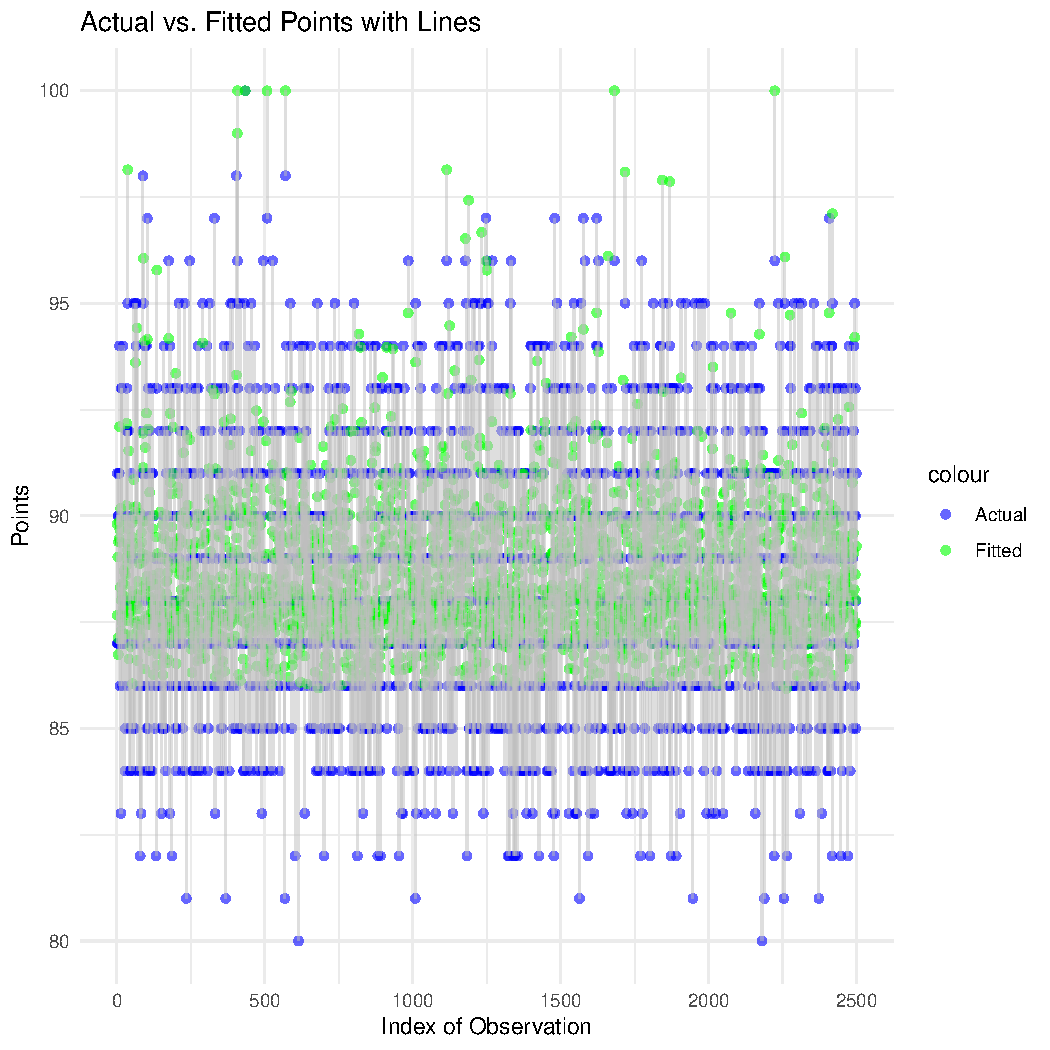
\includegraphics[width=0.5\textwidth]{imgs/Rplots-25.pdf}
	\caption{Actual vs Predicted Points}
	\label{fig:a_v_p_2}
\end{figure}

By using code:
\begin{verbatim}
	actuals_preds <- data.frame(Actual = wine_data$points, Predicted = fitted_values[, "Estimate"])
	correlation_accuracy <- cor(actuals_preds)
\end{verbatim}
We can get correlation table as shown in Table \ref{table:correlation}. This table shows a correlation coefficient of 0.6364308 between the actual and predicted points for wine points. This value indicates a moderate positive correlation, suggesting that the model's predictions align reasonably well with the actual points. However, the correlation is not very strong, implying that while the model captures some of the variability in the data, there remains significant room for improvement. A higher correlation would suggest a more accurate model that better captures the nuances in the data. This result underscores the need to perhaps refine the model or consider additional variables that could help increase the predictive accuracy.
\begin{table}[htbp]
	\centering
	\caption{Correlation between Actual and Predicted Points}
	\begin{tabular}{lcc}
	\hline
	 & \textbf{Actual} & \textbf{Predicted} \\
	\hline
	\textbf{Actual} & 1.0000000 & 0.6364308 \\
	\textbf{Predicted} & 0.6364308 & 1.0000000 \\
	\hline
	\end{tabular}
	\label{table:correlation}
\end{table}

Besides, by using code:
\begin{verbatim}
	min_max_accuracy <- mean(apply(actuals_preds, 1, min) / apply(actuals_preds, 1, max))
	rmse <- sqrt(mean((actuals_preds$Actual - actuals_preds$Predicted)^2))
	mae <- mean(abs(actuals_preds$Actual - actuals_preds$Predicted))
\end{verbatim}
We can calculate the Min-Max Accuracy, RMSE, and MAE metrics as shown in Table \ref{table:metrics}. The Min-Max Accuracy of 0.9786026 indicates that the model's predictions are generally within a narrow range of the actual points, reflecting a high degree of accuracy. The RMSE value and MAE value then show that the predictions of models would have low error rates.  These metrics all show that the model performs well in predicting wine points. And the prediction would have high accuracy and low error rates. However, there still have some room for improvement. We can enhance the precision and consistency of the predictions. The data of the Table \ref{table:metrics} is also visualized in Figure \ref{fig:Prediction_Accuracy_Metrics}.
\begin{table}[htbp]
	\caption{Performance Metrics}
	\centering
	\begin{tabular}{lc}
	\hline
	\textbf{Metric} & \textbf{Value} \\
	\hline
	Min-Max Accuracy & 0.9786026 \\
	RMSE & 2.3845760317167 \\
	MAE & 1.92613316721644 \\
	\hline
	\end{tabular}
	\label{table:metrics}
\end{table}

\begin{figure}[htbp]
	\centering
	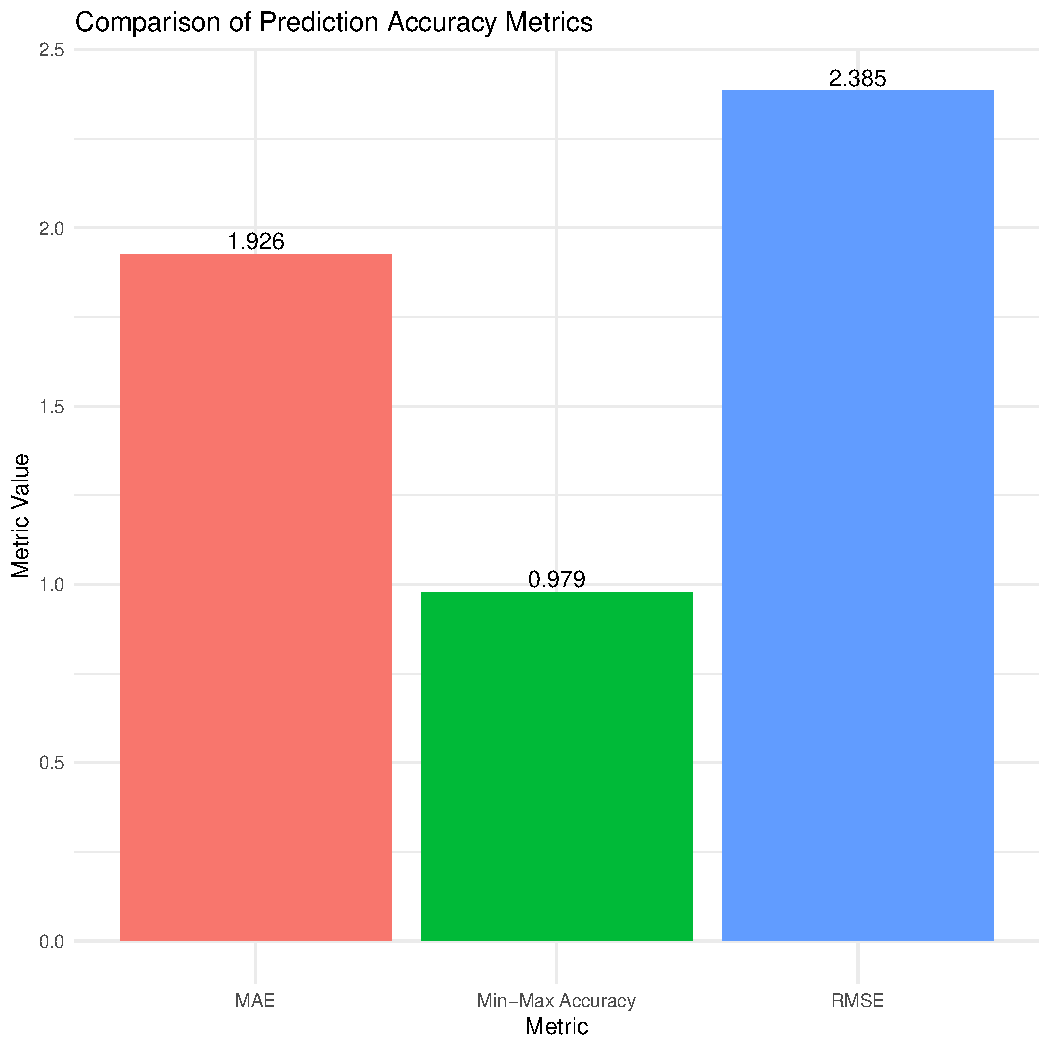
\includegraphics[width=0.5\textwidth]{imgs/Prediction_Accuracy_Metrics.pdf}
	\caption{Comparison of Prediction Accuracy Metrics}
	\label{fig:Prediction_Accuracy_Metrics}
\end{figure}

\section{Conclusions}\label{sec:conclusion}

\subsection{Summary of Results}

This study has build a Bayesian linear regression model to investigate how is the factors influence the wine ratings. The analysis of this study finally revealed some key points. Price and some sensory attributes such as Rich, Full, Firm, etc have significant positive effects on wine ratings, while the Soft, Crisp, Finish, etc. has a negative effects on wine ratings. The variety of the wine also has a minimal impact on the rating, which means that other factors have a much more important influence in wine quality. And this has affect the wine points. Besdies, the model achieved a moderate level of predictive accuracy, with a correlation of 0.6364308 between actual and predicted ratings, an RMSE of 2.3845760317167, an MAE of 1.92613316721644, and a 97.86026\% of Min-Max Accuracy. Density plots, hexbin plots, and actual vs. fitted plots, etc. has shown that while the model performs reasonably well, however, there still has some room for improvement in aspects such as reducing errors and enhancing prediction consistency.

\subsection{Evaluation of Methods}

By using the Bayesian linear regression approach in this study has several advantages. The model successfully identified the most influential factors affecting wine points. The Bayesian framework allowed for the incorporation of prior knowledge and the estimation of uncertainty in the model parameters. Diagnostic plots and performance metrics indicated that the model achieved a reasonable level of predictive accuracy.

However, there are also some limitations. The moderate correlation between actual and predicted ratings shows that the model may not fully capture all the factors in the data. There still have some room for improvement for predictive accuracy. Besides, the model assumes that there will have a linear relationship between the predictors and the response variable, however, this may not always be true in reality. 

Despite these limitations, the Bayesian linear regression approach is proved to be a useful tool for understanding the factors driving wine quality perceptions and providing actionable insights for stakeholders in the wine industry.

\subsection{Recommendations for Future Research}

To further improve the understanding of wine quality drivers and enhance the predictive accuracy of the models, future research could consider to explore non-linear modeling techniques, such as decision trees, random forests, or neural networks, which may better capture complex relationships between the predictors and the response variable. Also, incorporate additional variables, such as climatic conditions, soil characteristics, etc. may be a good idea. Besides, expanding the dataset to include wines from other regions and styles may also be helpful to the study. There is also possibility that the further study can be conducted based on the model we used since that it's available to be used in other similar studies and open source on GitHub. What's more, the study can be extended to consider the relationship between wine points and other factors, such as descriptions. There will be more factors can be extracted from the descriptions and they may have a significant impact on the wine points. By addressing these recommendations, future research can build upon the insights gained from this study and contribute to the development of more accurate and comprehensive models for predicting wine quality ratings.

\bibliography{refs}
\bibliographystyle{ieeetr}
\appendix
% \section*{Appendix}


\end{document}